%Template by Mark Jervelund - 2015 - mjerv15@student.sdu.dk

\documentclass[a4paper,10pt,titlepage]{report}



\usepackage[utf8]{inputenc}
\usepackage[T1]{fontenc}
\usepackage[english]{babel}
\usepackage{graphicx}
\usepackage{fancyhdr}
\usepackage{lastpage}
\usepackage{listings}
\usepackage{csquotes}
\usepackage{marvosym}
\usepackage[document]{ragged2e}
\usepackage[margin=1in]{geometry}
\usepackage{color}
\usepackage{datenumber}
\usepackage{venndiagram}
\usepackage{chngcntr}
% \usepackage{bera}% optional: just to have a nice mono-spaced font
\usepackage{xcolor}
\usepackage{amsmath,amsthm}
\usepackage{mathtools}
\usepackage{wrapfig}
\usepackage{multirow}
\usepackage[
    backend=biber,
    style=numeric,
    sorting=ynt
]{biblatex}

\newtheorem{theorem}{Theorem}




\colorlet{punct}{red!60!black}
\definecolor{background}{HTML}{EEEEEE}
\definecolor{delim}{RGB}{20,105,176}
\colorlet{numb}{magenta!60!black}

\lstdefinelanguage{json}{
    basicstyle=\normalfont\ttfamily,
    numbers=left,
    numberstyle=\scriptsize,
    stepnumber=1,
    numbersep=8pt,
    showstringspaces=false,
    breaklines=true,
    frame=lines,
    literate=
     *{0}{{{\color{numb}0}}}{1}
      {1}{{{\color{numb}1}}}{1}
      {2}{{{\color{numb}2}}}{1}
      {3}{{{\color{numb}3}}}{1}
      {4}{{{\color{numb}4}}}{1}
      {5}{{{\color{numb}5}}}{1}
      {6}{{{\color{numb}6}}}{1}
      {7}{{{\color{numb}7}}}{1}
      {8}{{{\color{numb}8}}}{1}
      {9}{{{\color{numb}9}}}{1}
      {:}{{{\color{punct}{:}}}}{1}
      {,}{{{\color{punct}{,}}}}{1}
      {\{}{{{\color{delim}{\{}}}}{1}
      {\}}{{{\color{delim}{\}}}}}{1}
      {[}{{{\color{delim}{[}}}}{1}
      {]}{{{\color{delim}{]}}}}{1},
}





\lstset{
  basicstyle=\ttfamily,
  columns=fullflexible,
  frame=single,
  breaklines=true,
  postbreak=\mbox{\textcolor{red}{$\hookrightarrow$}\space},
}

\addbibresource{bibliography.bib}


\DeclarePairedDelimiter\norm\lVert\rVert
\setdatetoday
\addtocounter{datenumber}{0} %date for dilierry standard is today
\setdatebynumber{\thedatenumber}
\date{}
\setcounter{secnumdepth}{0}
\pagestyle{fancy}
\fancyhf{}
\title{Masters Thesis}

\newcommand{\Z}{\mathbb{Z}}
\lhead{Masters Thesis}
\rhead{Mark Jervelund}
\rfoot{Page  \thepage \, of \pageref{LastPage}}
\counterwithin*{equation}{section}

\begin{document}
    \begin{titlepage}
        \centering
        \vspace*{9\baselineskip}
        \huge
        \bfseries
        Jepsen methods usage for ACID compliance in Hyperscale Cloud Frameworks \\
        \normalfont
        Mark Jervelund \\
        Mark@jervelund.com \\
        \vspace*{9\baselineskip}
        \normalfont
        
\includegraphics[scale=1]{logos/SDU_BLACK.png}
        \vfill\
        \vspace{5mm}
        Institute Of Mathematics and Computer Science, SDU \\

        %Date
        \textbf{\datedate} \\[2\baselineskip]
    \end{titlepage}

    \renewcommand{\thepage}{\roman{page}}% Roman numerals for page counter
    \tableofcontents
    \newpage
    \setcounter{page}{1}
    \renewcommand{\thepage}{\arabic{page}}


    \section*{Abstract}
    Databases allow modern society to store, manage, distribute, and receive data at a previously unprecedented scale. Working with data is standard practice for most businesses. Still, it is often done monotonically on a single node, where modern systems require more storage, lower latency, higher availability, and better performance than current systems allow. Distributing a data store in a manner that scales performance, storage, availability, and desired properties is no easy feat. In this thesis, I will present methods of verifying these properties and investigate how different frameworks solve this issue or often work around the issue in a way that aligns with the requirements of the systems. \\
    \vspace{5mm}

    Within the thesis framework, I will present methods of verifying the ACID properties, how they were solved in the past compared to how they are solved today, and what trade-offs some systems have made. I will also analyze modern database use cases and whether they require the ACID properties to satisfy their design goals.\\
    \vspace{5mm}


    The Thesis findings discover issues both within Service Fabric reliable Collections and within specifications of consistency Models. 
    Within Service fabrics, reliable collections, there are three issues: poor locks handling that cause significant abort rates and long transaction times that span up to 4 seconds per transaction,  and no use available optimizations allowed within the Repeatable read consistency model. 
    The results for the test show that Service Fabric expresses G0 and G1 -RT violations as well as as exponential abort rates in correlation with transaction length. and no guarantees with scaling beyond a single node, due to the under laying architecture that require the individual  implementations of a transaction manager and optimizer, however this might not solve the issue of deadlocking.
    Within the industry, the classifications and specifications of consistency models lack a usable standard that outlays what users can expect of the different models.
    A wide range of papers, outdated standards, and articles are currently used with mixed terminology, definitions, and specifications, which means that users cannot rely on documentation of how a given database or data store behaves.




    \chapter{Introduction}
    Highly Distributed systems are becoming commonplace as the world grows increasingly interconnected, faster-paced, more data-driven with higher expectations of user services and products. In these situations, the end-user expects availability combined with low- latency, reliability and, low cost. How do we guarantee this is a distributed system that spans the planet? Is it even possible to get both consistency and availability, and is it needed in most use cases?\\
    \vspace{5mm}

    Most people are familiar with how YouTube, Facebook, Google, and Reddit behave and the quirks they sometimes present.
    for example the YouTube video counter that got stuck at around 300 views and didn't update for a while. it was a side effect of a anti botting feature that caused it to stick, the system was designed to stop after the counter reached 300, but the counter would often go higher. This is an example of the system not being entirely consistent; most nodes were in the correct state of stopping the count when the number got larger than 300; however other nodes weren't consistent. Therefore the servers still counted the views even though they were supposed to have been sent to a different table that verified the views before considering them legitimate. Even though the number is still not consistent worldwide, this does not pose an issue as most people notice as a few seconds to a a minute delay when dealing with comments, views or likes or if the our comment isn't available to viewers around the world in real time and theirs aren't to us. 

    Many user-facing services aren't required to be fully consistent; however, there are use cases where not being consistent can have a severe impact. Strongly consistent transactions are of utmost importance when dealing with same types of data , such as financial data, automated or autonomous systems, and other areas where out of sync states might lead to issues.

    In the cases a lack of consistency would result in loss of life or significant loss of revenue. These situations require that no matter which server we are querying, it supplies the most recent data. If we receive stale data, we risk making an illegal transaction or an autonomous system making a wrong decision. This could be an automated trading system fetching stale data and making the wrong transaction, a bank withdrawal that might be overdrawing the users' accounts, or autonomous vehicles that might make decisions with stale data that can lead to fatal accidents. \\

    \vspace{5mm}
    How do we test and verify a given system's ACID compliance level? To understand this, we need to be familiar with the consistency levels and the intended behavior and anomalies they exhibit.\\
    
    In the following paper we investigate what consistent systems are, how they are defined, what anomalies they might exhibit and how are these verified. A test is also carried out on such a system, in this paper Azure Service Fabric will be analyzed. and the results show that even though it is consistent the implementation used is not without is drawbacks that highly limit the performance of the system.
    
Structure of the thesis.

    In Chapter 1, I will present ACID \& BASE, their constraints, faults in database systems, how they manifest themselves, the underlying causes, and the limits that ACID properties impose on a given system. BASE will be introduced to explain what relaxations are introduced to a system to gain desired properties and trade-offs.\\
    \vspace{5mm}

    In Chapter 2, I will introduce Jepsen, a Clojure framework\cite{jepsonio} developed by K. Kingsbury that allows for testing distributed systems. This is done by building a directed serialization graph (DSG) via querying the target system with carefully chosen queries for traceability and recoverability.  \\
    \vspace{5mm}

    Next, I will introduce Azure Service Fabric (SF). SF is a distributed container orchestration system made by Microsoft that allows for hosting services or containers. It includes a few different built-in subsystems, but the primary interest here lies in the aspect of SF's reliable containers and the claims Microsoft makes concerning the behavior of this datastore.\\
    \vspace{5mm}

    Afterward, I will present what modern database systems promise, the ACID properties they follow, the ones they relax or disregard, and the gain and trade-offs they suffer. Here the main focus will be on Service Fabric.\\
    \vspace{5mm}

    Subsequently,  I will demonstrate the attempt to implement and execute a Jepsen test against Service Fabrics reliable containers and compare these results to Microsoft's claims.\\
    \vspace{5mm}

    Finally, I will present the way ACID properties compare to modern use cases of databases. Do we need to follow them strictly, or can we disregard them in some use cases? What are the exceptions, and what is there to gain?\\


    \chapter{Database transaction models}

    Database and data store models can be categorized into two main groups, ACID and BASE, consistent or available.

    The underlying reason for both these is consistency limitations caused by the latency between nodes in the system. On a physical level, this results from the speed of light; in turn, a system cannot instantly distribute data between nodes. A systems availability limitation is the ability to respond to a given query: either wait for the changes to broadcast to all required nodes. Or reply via the best effort approach where each node responds with what information is available and then handle any write conflict down the line. Both models of designing the systems have their trade-offs which will be presented in this chapter.


    \section{ACID}
    The ACID Model of handling database transactions is considered monolithic by some. However, it still serves a vital and critical function for handling critical systems that require atomicity, consistency across the entire database, as well as reliability, and durability during hardware or software failure.\\
    \vspace{5mm}
    The ACID acronym is defined as follows in the DBMS book\cite{DBMSbook}.

    \begin{itemize}
        \item "A" stands for "atomicity," the all-or-nothing execution of transactions.
        \item "C" stands for "consistency." All databases have consistency constraints or expectations about relationships among data elements (e.g., account balances may not be negative after a transaction is finished). Transactions are expected to preserve the consistency of the database.
        \item "I" stands for "isolation," the fact that each transaction must appear to be executed as if no other transaction is performed at the same time.
        \item "D" stands for "durability," the condition that the effect on the database of a transaction must never be lost once the transaction has been completed.
    \end{itemize}

    ACID, therefore, offers strong consistency with rigorous handling of transaction isolation that prevents inaccurate data. This allows for designing a system to avoid operations on stale data, data loss, or "illegal" transactions. These faults will be presented later in the paper.


    \section{BASE}
    The BASE model allows the designing of a system where we value availability, throughput, and scalability. This can cause issues with stale data, dirty reads, overwriting data, and other undesired behavior. It can benefit some applications where overwriting old data isn't an issue, or the newest data version might not be required as long as it is available eventually. These databases are hugely beneficial for social media, logging, and other hyper-scale systems where consistency isn't needed.\\
    \vspace{5mm}
    The BASE acronym was defined by Eric Brewer\cite{brewer2000towards} as follows:

    \begin{itemize}
        \item Basically Available – Rather than enforcing immediate consistency, BASE-modelled NoSQL databases will ensure data availability by spreading and replicating it across the database cluster nodes.
        \item Soft State – Due to the lack of immediate consistency, data values may change over time. The BASE model breaks off with the concept of a database that enforces its consistency, delegating that responsibility to developers.
        \item Eventually Consistent – The fact that BASE does not enforce immediate consistency does not mean that it never achieves it. However, until it does, data reads are still possible (even though they might not reflect the reality).
    \end{itemize}

    The BASE model of databases often has a weak consistency where stale data is considered "OK" while offering a best-effort approach with approximate answers. It gains availability, performance, and it can be viewed as a relaxed way of handling the database side of things where the system database system is simpler and easier to modify the schema.


    \section{CAP theorem}

    Eric Brewer defined the CAP Theorem\cite{CAP}. It states that a distributed database system can't provide Consistency, Availability, and Partition Tolerance in a single system. Only two of these guarantees can be met.\\
    \vspace{5mm}
    It should be noted that the definitions of the terms differ from the definitions in ACID. They are all critical when it comes to distributed systems and their behaviors. Firstly, consistency in ACID is defined as constraints on the data. By the CAP consistency concept, ACID would follow sequential consistency as defined by Lamport\cite{lamport1993how}: "the program behaves as if the memory accesses of all processes were interleaved and then executed sequentially." While the consistency in CAP is defined as Atomic Consistency (also called linearizability), it is sequential with an added constraint of real-time ordering: "Unlike sequential consistency, linearizability implicitly assumes the notion of an observable global time across all processes. Operations are modeled by an interval consisting of the period of time between the invocation and response for the operation. Each operation is assumed to take effect instantaneously at some point within this interval". \cite{CSL-TR-95-685} \\
    \vspace{5mm}
    CAP states we can only have two of the three properties in any given data-share system. The three different options will be explained below.


    \begin{itemize}
        \item Consistency and Partition tolerance (CP) \\ A system that delivers consistency and partition tolerance but the trade-off here is availability. If a partition occurs in the system, the non-consistent nodes would have to be shut down or made unavailable to deliver consistent data. CP would cover majority protocols and most distributed databases. An example of a CP database would be MongoDB and Service Fabrics Reliable collections. These work by having partitions that contain a master and a set of replicates. The replicates simply follow the master's transaction log and apply it to their own data set. If the primary becomes unavailable, the Replicate with the most recent transaction log becomes the new master. During this switch, the partition becomes unavailable while the replicates catch up to the new master. This causes the network to remain consistent but limits availability. \\

        \item Availability and Partition tolerance (AP) \\ If a system foregoes consistency and delivers availability and partition tolerance, then in the case of a network partition between nodes, we keep serving from all nodes, but the system will serve stale data. It can also occur that rows contain different values due to multiple write operations on the various nodes. An example of an AP database would be Cassandra, where the CP has a master/replicate architecture. This would cover DNS, Caching systems. Cassandra uses a leaderless architecture; it does mean that there are multiple points of failure rather than a single one. It can be available and partition tolerant, but consistency isn't guaranteed as nodes are always available. In case of partitioning, the nodes will diverge while partitioned due to its Last Write Wins model and will first regain consistency once the network is healed. \\

        \item Availability and Consistency (CA) \\ Database delivers consistency and availability but doesn't allow for partitions of the network or nodes. This results in a single node or single cluster system as any system distribution introduces network instability and latency that would break the system. In this case, it would cover single-node/site databases and cluster databases as well as file systems as we, in practice, wouldn't have a distributed system that doesn't allow for partitioning as it would be unusable. But an example of this would be a single node database. PostgresSQL could be an example here; however, PostgresSQL does support replication, by becoming a CP style database. Some asterisks apply though as the system may not be consistent\cite{aphyrpostgres} as it doesn't behave as expected. \\
    \end{itemize}


    \newpage


    \section{Pretext to Consistency models.}

    \subsection{Availability}

    Availability refers to the guarantee a system promises doing the presence of network partitions.\cite{HighlyAvailableTransactionsVirtuesandLimitations}

    \begin{itemize}
        \item High Availability:
        \textit{
            Informally, highly available algorithms ensure "always-on" operation and guarantee low latency as a side effect. If users of a highly available system are able to contact a (set of) server(s) in a system, they are guaranteed a response; this means servers will not need to communicate with others synchronously. If servers are partitioned from one another, they do not need to stall in order to provide clients with a "safe" response to operations. This lack of fast path coordination also means that a highly available system also offers low latency; in a wide-area setting, clients of a highly available system need not wait for cross-data center communication. To adequately describe whether a transactional system is highly available, we need to describe what servers a client must contact as well as what kinds of responses a server can provide, especially given the possibility of aborts. Traditionally, a system provides high availability if every user that can contact a correct (non-failing) server eventually receives a response from that server, even in the presence of arbitrary, indefinitely long network partitions between servers \cite{CAP}. As in a standard distributed database, designated servers might perform operations for different data items. A server that can handle an operation for a given data item is called a replica for that item.}\cite{HighlyAvailableTransactionsVirtuesandLimitations}
        \item Sticky Available: \textit{In addition to high availability, which allows operations on any replica, distributed algorithms often assume a model in which clients always contact the same logical replica(s) across subsequent operations, whereby each of the client's prior operations (but not necessarily other clients' operations) are reflected in the database state that they observe. As we will discuss in Section 5, clients can ensure continuity between operations (e.g., reading their prior updates to a data item) by maintaining affinity or "stickiness" with a server or set of servers. In a fully replicated system, where all servers are replicas for all data items, stickiness is simple: a client can maintain stickiness by contacting the same server for each request. However, to stay "sticky" in a partially-replicated system,    where servers are replicas for subsets of the set of data items (which we consider in this paper), a client must maintain stickiness with a single logical copy of the database, which may consist of multiple physical servers. We say that a system provides sticky availability if, whenever a client's transactions are executed against a copy of database state that reflects all of the client's prior operations, it eventually receives a response, even in the presence of indefinitely long partitions (where "reflects" is dependent on semantics). A client may choose to become sticky available by acting as a server itself; for example, a client might cache its reads and writes. Any guarantee achievable in a highly available system is achievable in a sticky high availability system but not vice-versa.}\cite{HighlyAvailableTransactionsVirtuesandLimitations}
        \item Transactional Availability: \textit{Until now, we have considered single-object, single-operation availability. This is standard in the distributed systems literature    (e.g., distributed register models such as linearizability all concern single objects [41]), yet the database literature largely focuses on transactions: groups of multiple operations over multiple objects. Accordingly, by itself, traditional definitions of high availability are insufficient to describe availability guarantees for transactions. Additionally, given a choice to commit and abort responses— which signal transaction success or failure to a client—we must define transactional availability. We say that a transaction has replica availability if it can contact at least one replica for every item it attempts to access; this may result in "lower availability" than a non-transactional availability requirement (e.g., single-item availability). Additionally, given the possibility of system-initiated aborts, we need to ensure useful forward progress: a system can trivially guarantee clients a response by always aborting all transactions. However, this is an unsatisfactory system because nothing good (transaction commit) ever happens; we should require a liveness property.
        \vspace*{4mm}\\
        A system cannot guarantee that every transaction will commit—transactions may choose to abort themselves—but we need to ensure that the system will not indefinitely abort transactions of its own volition. We call a transaction abort due to a transaction's own choosing (e.g., as an operation of the transaction itself or due to a would-be violation of a declared integrity constraint) an internal abort and an abort due to system implementation or operation of an external abort. We say that a system provides transactional availability if, given replica availability for every data item in a transaction, the transaction eventually commits (possibly after multiple client retries) or internally aborts [9]. A system provides sticky transactional availability if, given sticky availability, a transaction eventually commits or internally aborts}\cite{HighlyAvailableTransactionsVirtuesandLimitations}

        \item Unavailable: A consistency model is considered unavailable if it is unable to make progress on any nodes doing a network partition, as it would break the consistency constraints required by a given model. These systems, therefore, have reduced scale-ability as they are often limited to running on a single node or cluster as any form of broader distribution would induce network issues that would pause the system or quit a brain split with subsequent data losses.

        \item Totally Available: A totally available system can be considered fully distributed and leaderless, such that any non-faulty node accepts traffic even doing a full partitioning. No guarantee  can be given on staleness as data can only be read from the node it was written to until the network is healed. If strict node persistence is maintained, "Read your Writes" can be maintained doing a network partitioning. Otherwise, there's is no guarantee provider that we can observe our own writes. 

    \end{itemize}

    \subsection{Transaction Anomalies \& Phenomena}
    Most consistency models are defined by what Phenomena they allow or prohibit. However, due to poor or loose definitions, there often exist multiple different definitions on each consistency model, as well as on many of the Phenomena, or simply the lack of a definition on some properties. Therefore an explanation of the different definitions and additions will be given below.\\

   ANSISQL99\cite{ansisql1999} defines three phenomena that are used to describe the different consistency models with transactional models. These are defined as follows:
    \begin{itemize}
        \item P1: Dirty Read — Transaction T1 modifies x. Another transaction T2 then reads x before T1 commits or aborts. If T1 then aborts, T2 has read a data item that was never committed and so never really existed.
        \item P2: Fuzzy or Non-repeatable Read — Transaction T1 reads x, then T2 modifies or deletes x and commits. If T1 then attempts to reread x, it receives a modified value or discovers that the data item has been deleted.
        \item P3: Phantom — Transaction T1 reads a set of data items satisfying some <search condition>. Transaction T2 then creates data items that satisfy T1's <search condition> and commits. If T1 then repeats its read with the same <search condition>, it gets a set of data items different from the first read.
    \end{itemize}


    However, these three Phenomena leave a lot of behavior of the models up to interpretation; therefore, Berenson et al\cite{Berensonetal}. from Microsoft wrote a paper on "A Critique of ANSI SQL Isolation Levels" in 1995 to include Read and Write Skew that defines data item constraint violations, where the ANSI models admit non-serializable histories. To resolve these issues, they wrote about a 4th phenomenon that describes item constraint violations. The exact definition is below: \\

\textit{(Data Item Constraint Violation). Suppose C() is a database constraint between two data items x and y in the database. Here are two anomalies arising from constraint violation}\\
    \begin{itemize}
        \item \textit{A5A: Read skew — Suppose transaction T1 reads x, and then a second transaction T2 updates x and y to new values and commits. If T1 reads y now, it may see an inconsistent state and produce an inconsistent state as output.
        In terms of histories, we have the anomaly:  } \\
         r1[x]...w2[x]...w2[y]...c2...r1[y]...(c1 or a1)
        \item \textit{A5B Write Skew — Suppose T1 reads x and y, which are
        consistent with C(), and then a T2 reads x and y, writes x,
            and commits. Then T1 writes y. If there were a constraint
            between x and y, it might be violated. In terms of histories:} \\
        r1[x]...r2[y]...w1[y]...w2[x]...(c1 and c2 occur)
    \end{itemize}
    This definition was later revised in Adya, \cite{Adya99weakconsistency} where the Dirty Write phenomenon is introduced to prevent non-serializable histories.


\subsection{Informal definition}

\begin{itemize}
    \item P0 (Dirty Write): w1(x) … w2(x)
    \item P1 (Dirty Read): w1(x) … r2(x)
    \item P2 (Fuzzy Read): r1(x) … w2(x)
    \item P3 (Phantom): r1(P) … w2(y in P)
\end{itemize}

    \subsubsection{P0 - Dirty Write}
     %TODO fix this section Dirty Write
        Suppose T1 modifies x and T2 further modifies x before T1 commits or aborts. If either T1 or T2 aborts, it is unclear what the real value of x should be. the preventive measure here should be that a transaction cannot overwrite changes made by an uncommitted transaction. Dirty write can also be defined as a locking mechanism in disguise that require the locking protocol in the history, that requires long-term locks for write and at least short term locks for read operations.


    \subsubsection{P1 - Dirty Read}
    %TODO fix this section Dirty Read.
        The preventative interpretation, P1, is more restrictive and requires that a transaction T2 must not read any object from an uncommitted transaction T1 (there is no abort or commit action for T1 between w1(x) and r2(x)); the lack of an abort or commit action in the condition simply means that all combinations of aborts and commits after r2(x) are disallowed.


    \textit{P1 ("Dirty Read"): suppose transaction T1 modifies a row. transaction T2 then reads that row before T1 performs a COMMIT. If T1 then performs a ROLLBACK, T2 will have read a row that was never committed and that may thus be considered to have never existed.} However, in the Microsoft paper, Berenson et al\cite{Berensonetal} it is observed that the ANSI specification allows multiple interpretations, one of which allows non-serializable histories. Here \cite{Adya99weakconsistency} is commonly used as it provides a concrete specification based on the ambiguous ANSI specification, that adds the Drity Write constraint defined by Berenson et al\cite{Berensonetal}.:
    
     P1 requires T1 to acquire a long write-lock and T2 to acquire (at least) a short-term read-lock,


    %TODO {Make example diagram}
    \subsubsection{P2 - Non-repeatable/Fuzzy Read}

   
    The second case of 'Non-repeatable read' is when S1 reads data that is changed by S2 and committed. So if S1 rereads the same data, it will have changed. This results in two equal, select statements returning different results.
    %TODO {Make example diagram}
    
     P2 requires the use of long read and write-locks; 


    \subsubsection{P3 - Phantom Read}

    The third and last type is phantom read which is a special case of non-repeatable read that occurs when S1 reads data where a where condition is used to specify what data we want. After this initial read, a second session S2 inserts data that meets S1's where condition and commits the data. When S1 issues a select statement with the same where condition, it finds new records. It is called Phantom Read because the new records seem to be of phantom origin.
    
    disallowing P3 requires acquisition of long phantom read-locks

    %TODO Make example diagram Phantom Read
    
\newpage
\subsection{The harsh reality}
    
    However in reality the above doesn't cover a lot of issues that can exist in DBMS systems. In Haixiang Li et al on COO\cite{li2021coo} 18 definitions on anomalies is brought 
\begin{table}[]
    \begin{tabular}{l|l|l}
        No & Anomaly, reference, year                        & Formal definition  \\ \hline
        1  & Dirty Write {[}1{]} 1992                        & $W_1 [x_1 ]...W_2 [x_2 ]...((C_1 or A_1) and (C_2 or A_2) in any order) $  \\
        2  & Lost Update {[}6{]} 1995                        & $  R_1 [x_0 ]...W_2 [x_1 ]...C_2...W_1 [x_2 ] $ \\
        3  & Dirty Read {[}1{]} 1992                         & $ W_1 [x ]...R_2 [x ]...(A_1 and C_2 in either order) $ \\
        4  & Aborted Reads {[}45{]} 2015, {[}2{]} 2000       & $ W_1 [x : i]...R_2 [x : i]...(A_1 and C_2 in any order) $  \\
        5  & Fuzzy/Non-repeatable Read {[}1{]} 1992          & $ R_1 [x ]...W_2 [x ]...C_2...R_1 [x ]...C_1 $  \\
        6  & Phantom {[}1{]} 1992                            & $ R_1 [P ]...W_2[y in P]...C_2...R_1 [P ]...C_1 $  \\
        7  & Intermediate Reads {[}45{]} 2015, {[}2{]} 2000  & $ W_1 [x : i]...R_2 [x : i]...W_1 [x : j]...C_2  $  \\
        8  & Read Skew {[}6{]} 1995                          & $ R_1 [x_0 ]...W_2 [x_1 ]...W_2 [y_1 ]...C_2...R_1 [y_1] $ \\
        9  & Unnamed Anomaly {[}38{]} 2000                   & \begin{tabular}[c]{@{}l@{}}$ R_1 [y]...R_2 [x ]...W_2 [x ]...R_2 [y]...W_2 [y]...C_2...R_3 [x ]...W_3 [x ]$\\$...R_3 [z]...W_3 [z]...C_3...R_1 [z]...C_1 $\end{tabular}      \\
        10 & Fractured Reads {[}16{]} 2017, {[}5{]} 2014     & $ R_1 [x_0]...W_2 [x_1 ]...W_2 [y_1 ]...C_2...R_1 [y_1 ] $ \\
        11 & Serial-Concurrent-phenomenon {[}12{]} 2014      & $ R_1 [x_0 ]...W_2 [x_1 ]...W_2 [y_1 ]...C_2...R_1 [y_1 ] $  \\
        12 & Cross-phenomenon {[}12{]} 2014                  & $ R_1 [x_0 ]...R_2 [y_0 ]...W_3 [x_1 ]...C_3...W_4 [y_1 ]...C_4...R_2 [x_1 ]...R_1 [y_1 ] $ \\
        13 & Long Fork Anomaly {[}16{]} 2017                 & $ R_1 [x_0 ]...R_2 [y_0 ]...W_3 [x_1 ]...C_3...W_4 [y_1 ]...C_4...R_2 [x_1 ]...R_1 [y_1 ] $ \\
        14 & Causality Violation Anomaly {[}16{]} 2017       & $ R_1 [x_0 ]...W_2 [x_1 ]...C_2...R_3 [x_1 ]...W_3 [y_1 ]...C_3...R_1 [y_1 ] $  \\
        15 & Read-only Transaction Anomaly {[}26, 43{]} 2004 & \begin{tabular}[c]{@{}l@{}}$ R_1 [x_0, 0]...R_1 [y_0, 0]...R_2 [y_0, 0]...W_2 [y_1, 20]...C_2$\\$...R_3 [x_0,0]...R_3 [y_1, 20]...C_3...W_1 [x_2, -11]...C_1 $\end{tabular} \\
        16 & Write Skew {[}6{]} 1995                         & $ R_1 [x_0 ]...R_2 [y_0 ]...W_1 [y_1 ]...W_2 [x_1 ] $   \\
        17 & Predicate-based Write Skew {[}27{]} 2005        & $ R_1 [P ]...R_2 [P ]...W_1 [y_1 in P]...W_2[x_1 in P] $  \\
        18 & Read Partial-Committed {[}44{]} 2019            & $ R_1[x] W_2[x] W_2[y] C_2 R_1[Y] C_1 $ 
    \end{tabular}
\end{table}





    
    https://arxiv.org/pdf/2109.06485.pdf base it on this paper ? ohh fancy !
%TODO Write Section about Faults and anomalies.

    \subsubsection{Long Fork}
%TODO Write Section about Long Fork.


    

    \subsubsection{Split Brain}
%TODO Write Section about Split Brain
The network is split into two or more parts where they each believe different truths,

    \subsubsection{Transient Anomalies}
%TODO Write Section about Transient Anomalies
    Process A writes x, then process B tried to read x, but x doesn't exist in the node, later process B is, however able to read A.

    \newpage


    \section{Consistency models}


    \begin{wrapfigure}{r}{0.5\linewidth}
        \centering
        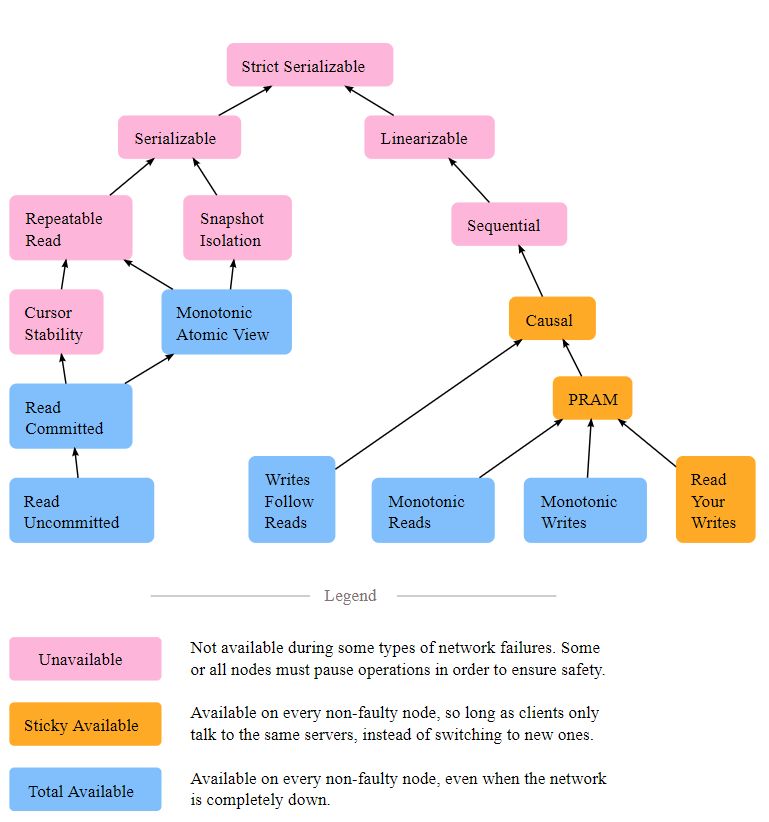
\includegraphics[scale=0.4]{images/consistency models.PNG}
        \caption{Picture from jepsen.io/consistency}
        \label{fig:jepsenioconsistency}
    \end{wrapfigure}

    For explaining the concepts within consistency, I will use a paper by Ballis et al. on "Highly available transactions"\cite{HighlyAvailableTransactionsVirtuesandLimitations} that contains a good model for presenting the different consistency models and their relation to other consistency models. A focus will be on Transactional models so not all of the BASE models are covered.\\

    \subsection{Strict Serializability}

    For a system to have Strict Serializability, it is required that the entire system operationally appears to occur in order, with regards to both the order and the real-time of the operations. Within the CAP theorem, this would be considered a CA system.\\
    \vspace{5mm}
    Formally Strict Serializability is defined as a Serviceable system that is compatible with a Time-dependent order.
    "A history is serializable if it is equivalent to one in which transactions appear to execute sequentially, i.e., without interleaving. A (partial) precedence order can be defined on non-overlapping pairs of transactions in an obvious way. A history is strictly serializable if the transactions' order in the sequential history is compatible with their precedence order." \cite{Herlihy1990Linearizability}\\
    \vspace{5mm}
    Here it should be clarified what is menat by the obvious way" is for a transactions A and B, that A proceeds B if A completes prior to transaction B's begin or in other words a Serializable system with the time constraint from Linearizability.

    SS cannot be totally or sticky available in the event of a network partition. In this case, some or all nodes will be stuck; this is due to the nature of the Strict serializable consistency model, where transactions operate on the system as a whole, as in the case of a partition in the distributed system, this is impossible. There can be cases where replicate nodes are partitioned from the primary nodes, and the primary nodes can continue with some degradation but where the replicas either shut down or serve stale data. In the case of primary nodes partitioning, the system would be unable to resume due to not being able to commit a given transaction to the entire system.


    \begin{table}[h]
        \begin{tabular}{l|l|l|l}
            T1   & T2   & T3   & T4   \\
            w(1) &      &      &      \\
            r(2) &      &      &      \\
            c    &      &      &      \\
            & r(1) &      &      \\
            & r(2) &      &      \\
            & c    &      &      \\
            &      & r(3) &      \\
            &      & w(4) &      \\
            &      & c    &      \\
            &      &      & r(1) \\
            &      &      & c
        \end{tabular}
        \caption{Transactions are ordered chronological in time, and executed as such.}

    \end{table}

    \subsection{Serializable transaction models}

    \subsubsection{Serializable}

    Serializability is a relaxation of the Strict Serializability consistency model that foregoes that real-time constraint. It defines systems where transactions occur in some total order. It is formally defined in the ANSI SQL 1999 spec as follows. "The execution of concurrent SQL-transactions at isolation level SERIALIZABLE is guaranteed to be serializable. A serializable execution is defined to be an execution of the operations of concurrently executing SQL-transactions that produces the same effect as some serial execution of those same SQL-transactions. A serial execution is one in which each SQL-transaction executes to completion before the next SQL-transaction begins." \cite{ansisql1999}\\
    \vspace{5mm}

    The above implies that Serializability of the transactions does not only apply to the objects in use but the system as a whole. This means that in the case of a network partition some or all notes will be stuck until the network is healed. Further, as no real-time constraint is enforced,  we can observe stale reads. This occurs when process A completes a write, then process B begins a read, and the read is not guaranteed to observe the write from process A.

    There is a further limitation of Serializable due to having no real-time constraint; SR allows pathological orderings. This allows a serializable database to discard, write, and increment operations that are never observed by executing them at the very end of the history. Furthermore, read operations can always return an empty state by placing the transaction at the beginning of the history. It should however be noted that most implementation does not take advantage of this.

    SR follows closely to S-SR regarding partition tolerance and availability doing partition and is therefore considered a CA database.

    \begin{table}[h]
        \begin{tabular}{l|l|l|l}
            T1   & T2   & T3   & T4   \\
            w(z) &      &      &      \\
            & r(z) &      &      \\
            &      &      & r(z) \\
            & w(y) &      &      \\
            &      &      & c    \\
            &      & r(y) &      \\
            & c    &      &      \\
            &      & w(h) &      \\
            r(x) &      &      &      \\
            c    &      &      &      \\
            &      & c    &
        \end{tabular}
        \caption{Transactions are ordered chronological in time and executed in a way that makes it possible for the operations to occur atomically such that they appear to have been executed in order transaction-wise. }
    \end{table}
    \newpage

    \subsubsection{Repeatable Read}

    Repeatable Read (RR) closely resembles the Serializable consistency model, however in RR we allow phantoms. This implies that if T1 reads a predicate like "select all from alarms with the newest timestamp," another transaction T2 is able to create or modify values within the predicate before T1 commits. So if the transaction T1 performs the read again, this predicate might not be stable.

    RR contains the above relaxation; however, this relaxation implies more than meets the eye. For example, repeatable read doesn't guarantee repeatable reads in the sense that we might consider. This is due to RR not requiring any real-time constraint; this allows for a situation where process A performs a write, and after process A completes process B performs a read. However, this read is not guaranteed to obverse the write from process A. Furthermore, as no per-process ordering of transactions is required, process A can write something and then fail to observe that write in a subsequent transaction.

    It should also be noted that RR allows for the same pathological ordering of operations as a Serializable database.

    \begin{table}[h]
        \begin{tabular}{l|l|l|l}
            T1            & T2            & T3   & T4   \\
            &               &      & r(y) \\
            &               &      & c    \\
            w(p$_1$ to y) &               &      &      \\
            r(p in y)     &               &      &      \\
            &               &      &      \\
            & w(p$_2$ to y) &      &      \\
            & c             &      &      \\
            r(p in y)     &               &      &      \\
            w(z)          &               &      &      \\
            c             &               &      &      \\
            &               & r(z) &      \\
            &               & w(x) &      \\
            &               & c    &
        \end{tabular}
        \caption{T1 shows an example of a valid transaction with a phantom, and T4 could be placed at the beginning of the history, returning the "empty" result. Both are valid transactions within RR.}
    \end{table}

    \subsection{Cursor Stability}
    Cursor Stability closely resembles repeatable read where RR locks the objects until committed. Cursor Stability locks the objects until the cursor moves on or until committed. This allows for different behavior depending on implementation but is formally defined by which phenomena it allows and which it prohibits.

    \cite{Adya99weakconsistency}\\
    \begin{itemize}
        \item G-cursor(x): the directed serialization graph, restricted to a single object x, contains an anti-dependency cycle and at least one write-dependency edge.
        \item g1:
        \begin{enumerate}
            \item G1a (Aborted Reads): A transaction observes an object (perhaps via a predicate) modified by an aborted transaction. Intuitively, transactions have to commit for us to read them.
            \item G1b (Intermediate Reads): A transaction observes an object (perhaps via a predicate) modified by a transaction that was not that transaction's final modification of that object. Intuitively, transactions have to finish before we can read them,
            \item G1c (Circular Information Flow): the Directed Serialization Graph of transactions contains a directed cycle consisting entirely of dependency edges. Intuitively, if transaction T1 is affected by T2, T2 can't be affected by T1.
        \end{enumerate}
    \end{itemize}
    Furthermore, since cursor stability is strictly stronger than read committed, it also prohibits the ANSI phenomena:
    \begin{itemize}
        \item P0 (Dirty Write): w1(x) … w2(x)
        \item P1 (Dirty Read): w1(x) … r2(x)
    \end{itemize}

    but allows:
    \begin{itemize}
        \item P2 (Fuzzy Read): r1(x) … w2(x)
        \item P3 (Phantom): r1(P) … w2(y in P)
    \end{itemize}


    %TODO Make diagram Cursor Stability

    \subsection{Snapshot Isolation}


    Snapshot Isolation behaves differently to any of the systems. It can be considered more as a \textbf{try: commit() catch: abort()} . We perform our transaction in an independent branch and commit/merge to the database on commit; if there are any conflicts with an already committed transaction, the transaction is simply aborted.

    Snapshot Isolation, like Readable Read, operates on an object level and allows for the same behavior. Items are stable once read; however, the predicate again isn't. We can fail to observe a previously committed transaction and place operations in arbitrary places in the transaction due to no Linearizability constraint. It also allows sub-operations to interleave. This can result in write skews, which allow transactions to read overlapping states, modify disjoint sets of objects, then commit; and a read-only transaction anomaly involving partially disjointing write sets.


    It should also be noted that there exist multiple versions of Snapshot Isolation, one being prefix-consistent snapshot isolation that enforces process-level transaction ordering, which prevents a given process from failing to observe a previous transaction; and another being parallel snapshot isolation that allows for total availability but this allows for long fork anomalies, as each node has its own transaction ordering.

    Formally Snapshot Isolation is defined by Berenson et al.\cite{Berensonetal}. as:

    \textit{… each transaction reads data from a snapshot of the (committed) data as of the time the transaction started, called its Start-Timestamp. This time may be any time before the transaction's first Read. A transaction running in Snapshot Isolation is never blocked attempting a read as long as the snapshot data from its Start-Timestamp can be maintained. The transaction's writes (updates, inserts, and deletes) will also be reflected in this snapshot, to be read again if the transaction accesses (i.e., reads or updates) the data a second time. Updates by other transactions active after the transaction Start-Timestamp are invisible to the transaction.
    \\
    When the transaction T1 is ready to commit, it gets a Commit-Timestamp, larger than any existing Start-Timestamp or Commit-Timestamp. The transaction successfully commits only if no other transaction T2 with a Commit-Timestamp in T1's execution interval [StartTimestamp, Commit-Timestamp] wrote data that T1 also wrote. Otherwise, T1 will abort. This feature, called First-committer-wins prevents lost updates (phenomenon P4). When T1 commits, its changes become visible to all transactions whose Start-Timestamps are larger than T1's Commit-Timestamp.}

    There also exist multiple other definitions from \cite{CeroneBernardiGotsman} and \cite{CrooksPuAlvisiClement}


    \begin{table}[h]
        \begin{tabular}{l|l|l|l}
            T1   & T2   & T3   & T4   \\
            &      &      & r(y) \\
            &      &      & c    \\
            w(y) &      &      &      \\
            r(y) &      &      &      \\
            &      &      &      \\
            & w(y) &      &      \\
            &      &      &      \\
            r(y) &      &      &      \\
            w(z) &      &      &      \\
            c    &      &      &      \\
            & a    & r(z) &      \\
            &      & w(x) &      \\
            &      & c    &
        \end{tabular}
        \caption{T1 and T2 contains a conflict that courses T2 to abort as T1 commits prior to T2}
    \end{table}



    \subsubsection{Monotonic Atomic View}
    The Monotonic Atomic view(MAV) model is a relaxation of snapshot isolation, it requires that effects by transactions are fully visible once read by other transactions, such that T1 may preform w(1), w(2), w(2), c. These 3 sub operations effects should all either be fully visible or not at all, so partial transactions aren't allowed. Formally this is defined by Bailis et al \cite{HighlyAvailableTransactionsVirtuesandLimitations}
    \textit{Under MAV, once some of the effects of a transaction Ti are observed by another transaction Tj, thereafter, all effects of Ti are observed by Tj. That is, if a transaction Tj reads a version of an object that transaction Ti wrote, then a later read by Tj cannot return a value whose later version is installed by Ti.}

    and by Adya et al\cite{Adya99weakconsistency} as prohibiting:
    \begin{itemize}
        \item G1b (Intermediate Reads): A transaction observes an object (perhaps via a predicate) modified by a transaction that was not that transaction's final modification of that object. Intuitively, transactions have to finish before we can read them,
    \end{itemize}

    Further since MAV is strictly stronger than Read Committed it also disallows the ANSI phenomena Dirty Write(P0), Dirty Read (P1) but allows Fuzzy Read (P2) and Phantom (P3)

    \subsection{Read Committed}
    The Read Committed transaction model is the first non-atomic transaction model where partial visibility of committed transactions is permitted. This however might lead to foreign key constraint issues, among other problems where required data joins are performed due to not yet visible values.


    Formally it is defined in ANSISQL1999\cite{ansisql1999} by disallowing P1
    \textit{P1 ("Dirty read" ): SQL-transaction T1 modifies a row. SQL-transaction T2 then reads that row before T1 performs a COMMIT. If T1 then performs a ROLLBACK, T2 will have read a row that was never committed and that may thus be considered to have never existed.} However, in the Microsoft paper, Berenson et al \cite{Berensonetal} it is observed that the ANSI specification allows multiple interpretations, one of which allows non-serializable histories. Here Adya et al.\cite{Adya99weakconsistency} is commonly used as it provides a concrete specification based on the unconcise ANSI specification.


    %TODO Make Diagram Read committed

    \subsection{Read Uncommitted}
    Read Uncommitted as defined by ANSI allows all behavior. However, this has been challenged by Berenson et al\cite{Berensonetal} where they argue that Read Uncommitted should disallow dirty writes. This is also the non-ANSI defacto definition as per Adya et al \cite{Adya99weakconsistency} which again provides a better definition based, on what can be interpreted from the loose definition in ANSISQL99\cite{ansisql1999}. It should be noted that due to the loose specification in ANSI, multiple mainstream interpretations exist.\\

    by the Aday's specification Read Uncommitted disallows
    \begin{itemize}
        \item Dirty Write(P0)
    \end{itemize}
    But allows
    \begin{itemize}
        \item Dirty read(P1)
        \item Fuzzy Read (P2)
        \item Phantom (P3)
    \end{itemize}

    \subsection{Non-transaction models (BASE)}
    The category of BASE transaction models aren't considering the ordering of transactions but rather the ordering of operations in real time.

    \subsubsection{Linearizable}
    Linearizablilty is the strongest single object consistency model, that requires operations to occur in a order consistent with real time, and the operations themselves should occur atomically. It should also be noted that linearzability is not tolerant to network partitions and should be considered a CA model according to the CAP theorem.

    it is formalized  in \cite{Linearizability} and later specified  in \cite{ConsistencyinNonTransactionalDistributedStorageSystems} where it's defined by 3 requirements


    \begin{itemize}
        \item Single Order (there exists some total order of operations)
        \item RealTime (consistent with the real time bound)
        \item RVal (obeying the single-threaded laws of the associated object's datatype)
    \end{itemize}

    %TODO Make Diagram Linearizable

    \subsubsection{Sequential Consistency}
    Sequential Consistency (SC) is a relaxation of Linearizability. Unlike Linearizability, SC is a concurrent model. Here the requirement is that all operations follow a total order and this order is consistent across all processes. However, since a Total order is required, the model is unable to tolerate partitions and some or all nodes will be unable to make progress. \\

    One of the phenomena SC allows is stale reads. All processes have to follow the same total order but as there isn't a strong constraint concerning how far a process may be behind or ahead and it may return an arbitrarily stale state. However, once a given node A observes some operations from a separate node B, A may never observe a state prior to B.

    Formally SC was defined by Leslie Lamport\cite{Lamport1979how}, however Viotti and Vukolić\cite{ConsistencyinNonTransactionalDistributedStorageSystems} formalized it into three requirements:
    \begin{itemize}
        \item SingleOrder (there exists some total order of operations)
        \item PRAM (the session order (the order of operations on each process) is a subset of the visibility order (what operations are visible to a given operation).)
        \item RVal (the order must be consistent with the semantics of the datatype)
    \end{itemize}

    %TODO Make Diagram Sequential Consistency

    % \subsubsection{Casual Consistency}
    % %TODO Write section on Casual Consistency
    % %TODO Make Diagram Casual

    % \subsubsection{Writes Follows Reads}
    % %TODO Write section on Writes Follows Reads
    % %TODO Make Diagram Writes Follows Reads

    % \subsubsection{Monotonic Reads}
    % %TODO Write section on Writes Follows Reads
    % %TODO Make Diagram Monotonic Reads

    % \subsubsection{Monotonic Writes}
    % %TODO Write section on Monotonic Writes
    % %TODO Make Diagram Monotonic Writes

    % \subsubsection{Read your writes}
    % %TODO Write section on Read your writes
    % %TODO Make Diagram Read your writes

    % Two of the consistency models were already mentioned in the previous section namely Atomic Consistency and Sequential Consistency. There exist two more models within common use, which are Causal Consistency and Eventual Consistency. They differ in the way the consistency is handled by all end up in the same state eventually.





    \newpage


    \chapter{Database Consistency testing}


    \section{Introduction}
    %TODO Write introduction Database Consistency testing


    \section{Modern Database systems, and the trade offs they make.}
    %TODO Write Modern Database systems  and the trade offs they make.

    Atomicity, and Isolation as we often write the data to a arbitrary node, that accepts after the data has been distributed outside of it's rack, availability zone or region. And where the newest timestamp then overrules all other written data without care of data on other nodes which can breaks Atomicity, and Isolation, as a check and set(CAS), or update statement might uses stale data and due to it's newer timestamp any data written in the meantime gets discarded. Solutions here might require waiting for full distribution of any data prior to the query executing, but this would drastically slow down the entire system. This does not factor in issues related to system faults though.
    """


    \section{Historically}

    Historically this was done with using a manually defined hand-coded set of patterns to check how a system behaves with regards to the isolation levels above like if some proven invariant hold, or if an anomaly is present in parallel  by inserting record x and y in two separate transactions and in two more transactions checking if we can observe x but not y, or y and not x, as this could show how the systems handle long forks and snapshot isolation, and more importantly if it supports it at all.

    These checks are generally quite efficient and run in polynomial time, but they only check for certain patterns and therefore don't give us the larger picture of where issues are present.  only cover a fairly limited set of configurations and isolation levels, and are defined on a system to system basis and no interchangeability is supporter.

    This means that this has been a giant scope project where case by case tests are predefined and where we only test for certain scopes, which more importantly mean that tests have been done but the test coverage haven't been perfect and a lot of anomalies are never detected.

    %TODO write more on the Historically {Need to add some more to this section, add examples are past test, diagrams, papers etc}


    \section{Jepsen}
    "
    Jepsen is an effort to improve the safety of distributed databases, queues, consensus systems  (...) exploring particular systems' failure modes. In each analysis we explore whether the system lives up to its documentation's claims.
    "\cite{jepsonio}
    \\
    \vspace{5mm}

    Going from the above quite Jepsen is a way that allows us to check whether a given database system lives up to the requirements and premises that are given, and in a world where distributed, hyper scale or even planetary scale systems are becoming the norm the way data storage is done is required to behave in an expected manner, the reason that expected manner is used rather than correct manner is that we may allow certain faults to occur and eventual consistency to allow for higher throughput applications and that some data may only be required locally as to consider a transaction complete even in the case where some undesirable conditions occur, but these are tolerated to a certain extent. \\
    \vspace{5mm}
    Two different examples of this is the YouTube 301 views that happened around 2015, where the number of views weren't globally distributed the right away, while comments and likes were. This meant two things. \\

    Comments were available globally in real time, while views would also commit globally doing low load times, or off hours to maximize utilization of resources.\\
    \vspace{5mm}
    Another more modern scenario where the real time data distribution and correctness is of the utmost importance is within transactions in the finance industry,  where we only want to consider a financial transaction committed once all shards of this data is replicated and the 'old' balance is no longer available, otherwise we could reach a condition where worst case a client is able to draw a negative balance on their account or where one of the transactions isn't recorded as only one of the two transactions is recorded.\\


    \section{State of the art.}

    The state of the art is Jepsen, or rather one of the state of the Art projects.

    Jepsen supports quite a few different modules but the most powerfull features goes by the name Elle, inferring isolation anomalies from Experimental Observations. \\
    \vspace{5mm}
    The way this works is by inferring a dependency graph between client side observations and the database version history. This is done by carefully selecting database objects and operations such that the database reads reveals information about the version history.\\
    \vspace{5mm}
    This means that Elle is able to reveal any anomaly and provide a concise explanation as to why a fault occurred with information of what conditions were present to cause this fault to occur. Using this information we are able to say how a system behaves, what level of isolation and which behavior we'll see as well as what promises the system makes and how does promises are reflected in reality.\\
    \vspace{5mm}

    And these things can be manifested in multiple ways, some cases are as mentioned earlier in the paper accepted as eventually consistency and performance is valued higher or some applications where loosing some data points are acceptable to allow for higher write throughput.\\
    \vspace{5mm}

    And the same does for stale, dirty, non-repeatable and phantom reads aren't an issue. This could be on hyper scale social networks where if you see something that was deleted, or if the newest posts, comments and likes aren't distributed across the all notes, but they will eventually. But this is a trade off that is done to allow for much higher write performance as the chance a user is making chancing to the same page on two different nodes/clusters are minimal and the required performance drop required to facilitate the guarantee that all data is always up to date would mean that the system wouldn't scale at the rate it's required, this also brings up another interesting topic, approximate programming, where a program doesn't always have to return the correct output, but if we can see a magnitude speedup of a program and accept a faulty result rate of a few \%, then the cost saving and capacity increase could very much be worth it. This could be in the case of Netflix and amazon recommencing products and services, it doesn't have to be perfect and maybe sometimes the result is wrong but if it means we're able to serve a lot more customers before having to degrade services or maybe having it as a step in the service degradation levels to support as many users as possible. \\
    \vspace{5mm}
    But a lot of this lay outside the scope of this thesis but it's also a super interesting field that will probably see grow in the next decade.


    \subsection{Elle}
    
    
    Elle is a consistency checker and generator available in Jepsen. It supports a few different methods 
    
    Elle is the one of the Jepsen Consistency checkers available in jepsen, other exist but for all intents and purposes Elle should always to used. 
    Introduction to Elle
    ...
    What it aims to solve
    ...
    DSG
    ...
    Checker
    ...
    Generators
    ...
    TXN
    ...
    
        %TODO move these to BIB file and write this section
    % K. Kingsbury. Knossos.
    % https://github.com/jepsen-io/knossos, 2013-2019.

    % G. Lowe. Testing and Verifying Concurrent Objects.
    % Concurrency and Computation: Practice and
    % Experience, 29(4), 2017

    % J. M. Wing and C. Gong. Testing and Verifying
    % Concurrent Objects. Journal of Parallel and
    % Distributed Computing, 17(1-2), 1993.

    % P. B. Gibbons and E. Korach. Testing shared
    % memories. SIAM Journal on Computing, 26(4), 1997

    % S. Burckhardt, C. Dern, M. Musuvathi, and R. Tan.
    % Line-up: A Complete and Automatic Linearizability
    % Checker. PLDI '10, 2010.
    
    
    
    

    \section{Past Jepsen tests}
        Finding in past Jepsen test.
    \subsection{Cassandra}
    A test was done on Cassandra in 2013 that showed some interesting behavior, with interesting names such as doomstones, and that doing conflicts a lexicographically bigger value is winning. such that separate parts of separate transactions might end up in the database. .\\
    \vspace{5mm}
    Casandra itself is built on a hash ring via a distributed hash table like Service Fabric. but unlike most other database it uses timestamp based last write wins. this allows for extremely high performance but also at the cost of being highly sensitive to clock skew.\\
    
    In the test on Cassandra it was found that:
    \begin{itemize}
        \item doing a single key heavy write operations Losing 28\% of committed data and fails linearizable by any definition.
        \item Doing Write conflicts roughly 1 in 200 rows end up being corrupt due to poor handling time time where milliseconds are used with 3 zeros at the end instead of microseconds.
        \item \textit{No. Cassandra lightweight transactions are not even close to correct. Depending on throughput, they may drop anywhere from 1-5\% of acknowledged writes–and this doesn’t even require a network partition to demonstrate. It’s just a broken implementation of Paxos. In addition to the deadlock bug, these Jepsen tests revealed \#6012 (Cassandra may accept multiple proposals for a single Paxos round) and \#6013 where a insert is rejected but committed anyway. (unnecessarily high false negative probabilities).}
    \end{itemize}

    https://aphyr.com/posts/294-call-me-maybe-cassandra


    \subsection{Postgres}
    
    
    
    \begin{itemize}
        \item \textit{Users should be aware that PostgreSQL’s “repeatable read” is in fact snapshot isolation—a fact long-understood in the PostgreSQL community and previously reported by Kleppmann. Since G2-item is prohibited under common formalizations of repeatable read, users may have designed applications assuming this held true for PostgreSQL. In this case, users may wish to run selected transactions under serializable isolation instead, add explicit locking, or redesign those transactions such that they are no longer sensitive to G2-item.}
        \item \textit{It appears that no version of PostgreSQL has ever guaranteed serializability. Users should be aware that concurrent update and insert transactions may exhibit G2-item. High-contention workloads are especially susceptible. The PostgreSQL team has written tests to reproduce the problem and is evaluating a patch; we recommend upgrading once the next minor release becomes available.}
    \end{itemize}
    https://jepsen.io/analyses/postgresql-12.3

    \section{related work to Jepsen}
    
    %TODO move these to BIB file and write this section
    % K. Kingsbury. Knossos.
    % https://github.com/jepsen-io/knossos, 2013-2019.

    % G. Lowe. Testing and Verifying Concurrent Objects.
    % Concurrency and Computation: Practice and
    % Experience, 29(4), 2017

    % J. M. Wing and C. Gong. Testing and Verifying
    % Concurrent Objects. Journal of Parallel and
    % Distributed Computing, 17(1-2), 1993.

    % P. B. Gibbons and E. Korach. Testing shared
    % memories. SIAM Journal on Computing, 26(4), 1997

    % S. Burckhardt, C. Dern, M. Musuvathi, and R. Tan.
    % Line-up: A Complete and Automatic Linearizability
    % Checker. PLDI '10, 2010.

%TODO write introduction to writing jepsen test






    \newpage


    \chapter{Modern Datastores}


    \section{Introduction}

    The thesis will primacy focus on Service Fabrics but investigation into other data stores is also done to allow comparisons and investigation into what different models affect the behavior of the database systems.


    \section{Service Fabric}

%    https://www.microsoft.com/en-us/research/wp-content/uploads/2016/02/tr-95-51.pdf
%
%    https://docs.microsoft.com/en-us/azure/service-fabric/service-fabric-reliable-services-reliable-collections

    \subsection{Introduction}

    Service Fabric (SF) is a presented as a distributed systems platform something akin to Kubernetes (K8S), where the user is able to build, deploy and scale micro services and containers. One of the key points presented by on Azure Service Fabric is that you're able to run stateful services. It's presented by Microsoft as the backbone of their core services and data stores.\\
    \vspace{5mm}

    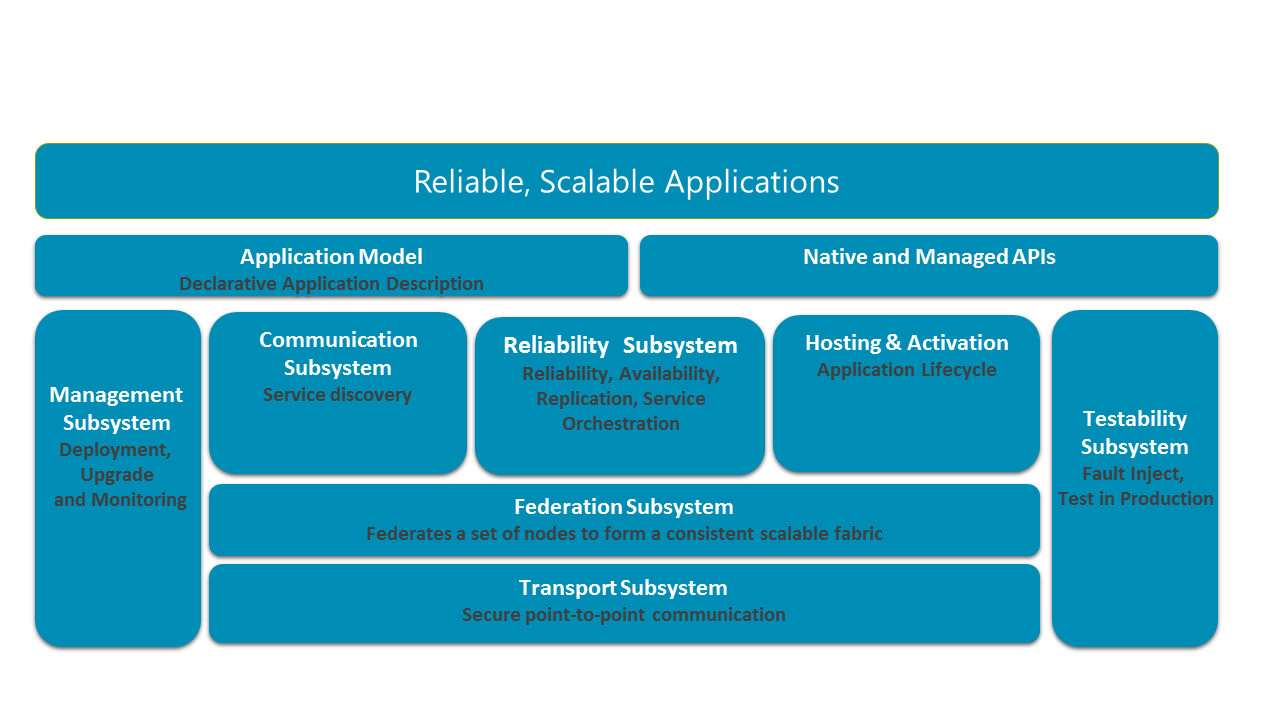
\includegraphics[scale=0.5]{images/service-fabric-architecture.png}

    \subsection{System Architecture}

    The architecture behind Service Fabric is built via a layered approach, that by Microsoft's words allows developers to write applications that are highly available, saleable, manageable and testable. These layers are built on 5 Core and 2 supporting subsystems. Our main interest lies within the reliable collection so I will only be investigating the layers and services that lay below this.\\
    \vspace{5mm}

    \subsubsection{Transport subsystem}
    %TODO these might be serving the same purpose and the documentation might just be odd.
    The lowest layer in the core stack that provides secure communication within the cluster itself and between the cluster and clients. This functionality is provided via point to point communication channels that support one way and request reply patterns, in other terms UDP and TCP. This also provides basis for broadcast and multicast within the cluster. Security is handled via wither windows security or x509 certificates. \\
    \vspace{5mm}

    \subsubsection{Federation subsystem}

    The next subsystem in the stack is the Federation subsystem that uses the communication channels provided by the transport subsystem to gather the nodes in the system into a unified service fabric cluster, and provides system primitives that allow for Failure detection, leader Election and consistent routing within the distributed system.\\
    \vspace{5mm}

    The core of the subsystem is built around a SF-ring that was developed internally at Microsoft in the early 2000s, where both keys and nodes are mapped to a point in the ring, with keys being owned by the node closest to it in the ring. where each node also uses this ring to keep track of its immediate successor and predecessor nodes that it stores in a Neighborhood set, this set is then used by the Federation layer to run consistent membership and failure detection. Nodes also maintain long distance routing partners that are used for consistent routing.\\
    \vspace{5mm}

    The membership and Failure detection is doing using tow key design principles.\\
    \vspace{5mm}

    Strongly Consistent membership and Decoupling Failure Detection from Failure Decision\\
    \vspace{5mm}

    \begin{itemize}
        \item \textbf{Strongly Consistent membership} All nodes must monitoring a given nodes status must agree on weather the node is up or down. for use in the SF ring this means that the all nodes on the node's Neighborhood set must agree on its status.
        \item \textbf{Decoupling Failure Detection from Failure Decision}: failure detection protocols can lead to conflicting states, therefor the decision is decoupled from detection.
    \end{itemize}
    \vspace{5mm}

    To solve the issues of decoupling the failure detection and decision that is used need distribute all decisions to the responsible nodes and ensure that these decisions are all done in a consistent and reliable manner. For the monitoring aspect of this s distributed monitoring and leasing solution is implemented by SF. This implementation solves this via Lease Renewal Request(LR) and LRack. A node is simply required to maintain valid leases from all of it's monitors and these leases have to be renewed every lease period, this leasing period is calculated based on round trip times but is typically around 30 s. If a node fails to renew any of these leases it considers moving itself from the set, and if a monitor misses a request from It it considers marked the monitor as failed. both these decisions need to be approved by a Arbitrator group. if a node fails to receive a LRack within a timeout based on round trip time it repeats the LR until it receives a LRack, Due to the nature of the SF-ring these monitor relations are symmetrical, but this Lease protocol is still run independently, there are however other cases, It a node fails the renewal process is stops renewing leases to any other nodes, or if a node detects a other node as having failed it stops sending renewal request to it. these 2 cases have the potential to cause inconsistencies if they were operating alone, however decision of deciding if a node is down or up is up to the Arbitrator group, which maintains consistent memberships. \\
    \vspace{5mm}

    The decision of deciding on failures is preformed by the Arbitrator group this is separate from the neighborhood set. They operates independently and have two it has two ways of deciding if a given node has failed. The way that the groups stays consistent when members join or leave the group is that when a Arbitrator joins the set, it initially rejects all requests in the first t seconds, this is done to prevent new Arbitrator making conflicting decisions with the excising nodes, and to prevent failed nodes to exist in the distributed membership protocol. this ensures that detected nodes leave before being forgotten.\\
    \vspace{5mm}

    \begin{enumerate}
        \item X detects Y as failed and sends fail(Y) to the arbitrator
        \item The arbitrator Ads Y to a recently failed list and sends ack(fail(y)) containing a timeout for Y to X, if The arbitrator already marked X as having failed and ignores the request,
        \item If X receives this request it waits for the TO to claim Y's area of the ring. and if re receives no response within the timeout it leaves itself.
    \end{enumerate}

    If a node is already in the recently failed list it returns the same response as the the first reporter except it calculates in time since first detection so the portion of the ring is claimed by the neighbors at the same time. This also means that the routing can continue after to with a laxity added. as all routing request for a node are added to a queued if a node is marked a failed. and the queue is released after TO+laxity that allows a neighboring node to claim that part of the ring and allows to these routing request to be preform when by it's successors.\\
    \vspace{5mm}

    If the case of two nodes report each other as failed the conflict is resolved either by majority, such that node that was reported first to the most Arbitrators leave or an alternate variant that heals the membership if both nodes are healthy and allows both to stay. in cases of network congestion or partitions that result in multiple nodes detection each other as failed, in traditional distributed hash tables this can result in inconsistencies in the membership lists or ring. \\
    \vspace{5mm}

    The implementation in SF is presented as being failure tolerant towards cascade failures as the decision isn't made by the detectors themselves but by arbitrators. an example is used that if a given node is only dependent by it neighbors and ½ of them fails to renew it's lease it will leave itself. No mention here is written about how the node handles being fragmented into two partitions and rejoined later, but mentions that this approach scales to entire data centers, no mentioned about how it scales across regions or outside of data centers.\\
    \vspace{5mm}

    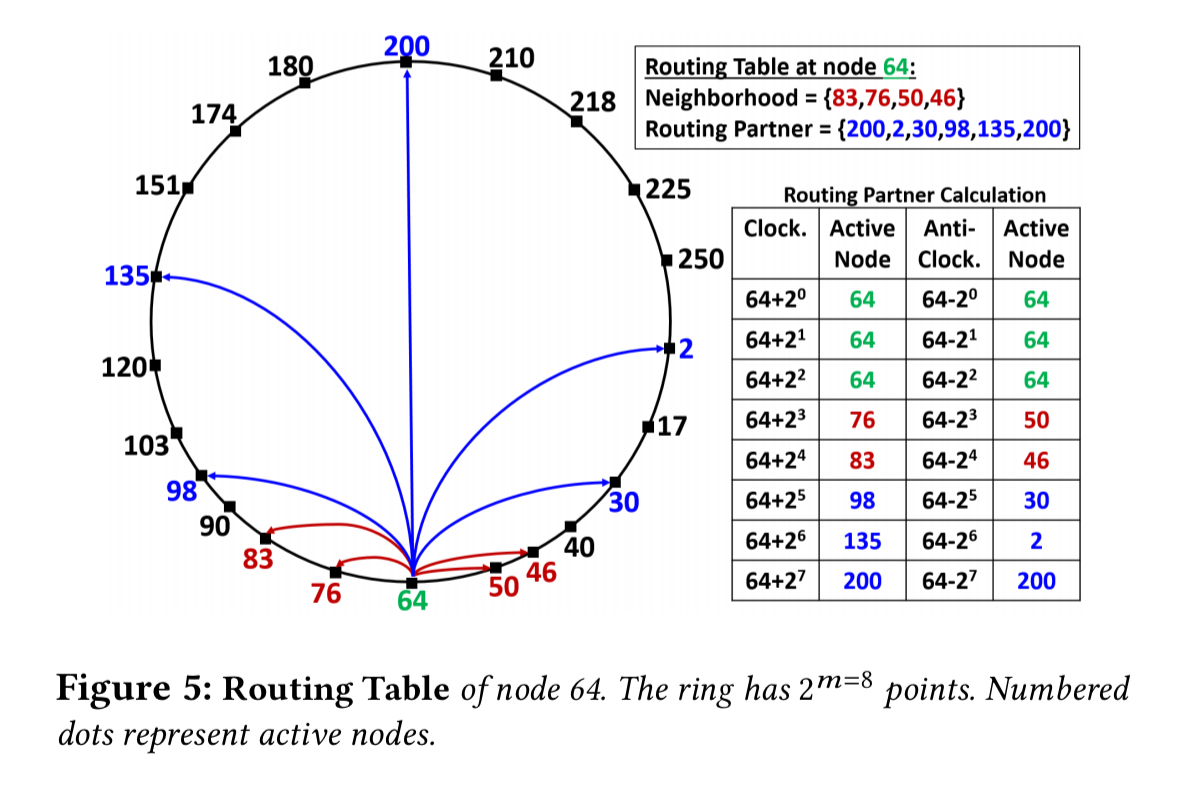
\includegraphics[scale=0.3]{images/servicefabric-fig-ring-topology.jpeg}

    SF-Ring and consistent routing.(need to rewrite/reword this to a more coherent sentence.)

    The Distributed Hash table used for service fabric routing is a evolution of SF-ring that was developed within Microsoft in the 2000s. The routing used offer symmetry and due to this it allows bidirectional routing that allow for lookup and routing via binary search, this allows SF to in practice routes message around the ring in a fast manner, with multiple routing options in that there always exists 2 routing partners on either side of the destination that both helps distributed the load and is able to route even with stale routing tables. Initially all packages were routed using this method however this has changed over the years, today the hash table is used to build a routing table and maintain it when a new node is added to the cluster, and ti route message to virtual addresses. After discovery a direct route is used via the destination IP address. \\
    \vspace{5mm}

    Routing tables work differently depending on the size of the cluster. however it is able to route in two ways, If the size of the routing table is smaller then the number of nodes a direct route is used, if there exist more nodes in the cluster then the routing tables it stitches to routing via routing tables to reduce memory consummation but causing an increase in time complexity to O(Log(n)) from O(1)\\
    \vspace{5mm}

    Routing Tokens.
    %TODO I was unable to find information on this precisely is handled however from the wording in the paper the initially split would be 50/50 and a third node would be 50/25/25? is it split evening it 33/33/33 but a Fourth node would be 22/22/22/33 that would cause unbalance unless some shifting is done
    Each node owns a token that includes a portion of the routing token it is responsible for. The sf-ring protocol ensures two properties, That each token is only owned by one node at any given time, and that eventually every token is owned by 1 node. This is ensure in the way that SF handles nodes joining and leaving the ring. Initially the bootstrap node owns the entire ring. after this inertial bootstrap node any joining node will split the ring segment between them.\\
    \vspace{5mm}


    These routing tokens are also used for leader election, Simply the owner of a given key is the owner.

    \subsubsection{Reliability subsystem}
    The reliability subsystem is in charge of load balancing, replication and availability. These three aspects are provided via 3 services, Failover Manager, Naming and Resolution, and a Placement and Load Balancer service.\\
    \vspace{5mm}

    The Failover Manager is running as stateful service, that has a instance running on each node in the cluster, that provide 3 actions, start a replica, move a replica, reconfiguration.\\
    \vspace{5mm}

    \begin{itemize}
        \item \textbf{Create a replica} Create a new replica when instructed by the PLB
        \item \textbf{Move a replica} migrate a replica when instructed by the PLB to a different node.
        \item \textbf{Reconfiguration} If a primary replica becomes unavailable to promotes a secondary as the new primary, in case the old primary comes back only it is demoted to secondary.
    \end{itemize}

    A service called Failover Master Manager is also running that is able to restart the failure manager via a cached state in case it fails. in case the master fails it is able to rebuilt its state via the SF-ring, the Master Failover manager is running on the node who's token range contains ID0.\\
    \vspace{5mm}

    The naming and resolution service maps instance names to endpoints that running services are listening on, this also allows for consistent routing from outside of the cluster via URI that doesn't change over a their lifetimes.\\
    \vspace{5mm}

    The Placement and Load Balancer(PLB) service is stateful and is in charge of placing replicas and instances of services at nodes and ensure even load throughout the cluster. they claim that unlike other solutions where services are hashed onto the ring in SF the PLB explicitly assigns each services replicas Primary and Secondaries to nodes in the Ring. it continually monitors the cluster for available resources to both assigned and migrate services to underutilized nodes and migrates services away from a node that is about to be upgraded or is overloaded due to a long workload spike.\\
    \vspace{5mm}

    The technique used for selecting placement of nodes is done via Simulated Annealing, as it is presented to provide a near optimal solution as to where services can be placed, This way the system is modeled is via resource use in the system where a even load is desired, but some constraints need be met such as fault tolerance, avoiding replica co-location and some service might have strict set of nodes to run on. \\
    \vspace{5mm}

    \subsubsection{Reliable Collections}

    Reliable collections provide stateful services in Service fabric via Reliable Directories and reliable Queues that are available for C\# and java programming, and are promised to be:
    \begin{itemize}
        \item Available and Fault-tolerant via replication,
        \item Persistent via disk
        \item Efficient via asynchronous via API that are non blocking.
        \item Transnational via APIs with ACID semantics.
    \end{itemize}

    One of the key differences between storage systems build on SF and other highly-available systems is that states are kept locally in the replica while also being made highly-available, this causes most reads to be local.\\
    \vspace{5mm}

    Writes are relayed from the primary replica to secondary replicas via passive replication and are considered complete when the majority of secondaries acknowledges it. the relaxations allow an application to achieve weaker consistency by relaxing where a read can go, eg: always read from primary to read from secondary. \\
    \vspace{5mm}

    SF is presented as the only "self-sufficient microservice system that can be used to build a transactional consistent database which is reliable, available, self-*, and upgradeble because the lower layers assure consistency"\cite{SFpaper} \\
    \vspace{5mm}

    \paragraph{Consistency models/isolation levels}
    SF reliable collections promise two Select-able consistency models that the user can pick. Repeatable Read and Snapshot isolation. eg there is no promise about Serializability of the transactions.\\
    \vspace{5mm}

    \begin{table}[h]
        \centering
        \begin{tabular}{l|l|l}
            & \multicolumn{2}{c@{}}{\text{Role}} \\
            \text{Operation}   & Primary         & Secondary \\
            Single Entity Read & Repeatable Read & Snapshot  \\
            Enumeration, Count & Snapshot        & Snapshot
        \end{tabular}
        \caption{isolation level defaults for Reliable Dictionary and Queue operations.}
        \cite{SF_RC_Transactions}
    \end{table}


    \section{Programming for Service Fabric}
    
    Implementing services for SF is written in ether Java or .Net. The documentation for Java is highly lacking so .Net was chosen. 
        ...
    It was discovered that the documentation for .Net was also highly lacking, outdated in other ways had issues so a lot of issues was figuring it out from the ground up. Implementation features, 
    ...
    testing how they behaved and learning from there. This also meant that a lot of time was spent learning .Net and the specific frameworks used in the implementations.
    ...
    The .Net code was fairly straight forward to learn while the Service fabric and other libraries where more of a challenge to decipher and implement. 
    ..
    this was further escalated by poor support for development on non Windows platforms that require manual everything and no feedback loop from deployment. 
    ...
    Web application in SF are programming using Model View Controllers (MVC) and the SF framework for the under laying reliable collections 
    
    
    
    Dotnet, lack of debugging tools, non features parity between platforms. etc
%TODO write Programming for Service Fabric



    \section{Comparison}
%TODO write Comparison between the 3 datastores
    In many of the papers published by Microsoft a lot of comparisons are made to Cassadra, Redis and Dynamo. Therefore, comparisons will be made to two of these as they are comparable in a lot of aspects. The investigation won't be as deep as with SF but investigation of consistency and failure modes will be be done.
    
    
    
    \subsection{Cassadra}
    
    Facebook database product made opensource,
    
    Ring via hash table
    
    Last write wins
    
    Leaderless
    
    scalability
    
    Clock skrew issues
    
    Handling of conflicts
    
    sensitivity to time desync
    
    possible solution ?
    
    usecases
    
    

    \subsection{Redis}
%TODO write section on Redis

    \subsection{Dynamo}
%TODO write section on Dynamo


    \section{Comparison}
%TODO write Comparison between the 3 datastores
    In many of the papers published by Microsoft a lot of comparisons are made to Cassadra, Redis and Redis. Therefore, comparisons will be made to these as they are comparable in a lot of aspects. The investigation won't be as deep as with SF but investigation of consistency and failure modes will be be done.


    \chapter{Jepsen Test on Service Fabric Reliable collections}


    \section{Introduction}

    The Goal of the thesis was to attempt to preform a Jepsen test on Service Fabric with it's reliable collection subsystem that powers a lot of the services in Azure and being the target of this endeavor. 
    In this chapter we will present the design, and implementation and revisions of the testomg suite-
    To perform such a test we need to build up both a testing suite, APIs and libraries to allow for a connection between the Jepsen service and the Service Fabric core components. Therefore a few different applications and services need to be learnt, understood, designed, implemented, tested, executed, and at last the data generated from this can be analyzed.
    \begin{itemize}
        \item Learning the required tools to implement the services and applications in the first place. C\#, Clojure, and Service Fabric itself as well as reliable collections and lastly Jepsen itself.
        \item Understanding the problem, requirement, topology, architectures and how we want to test these things.
        \item Designing the Services, Libraries, APIs, testing suite, and the infrastructure and networking of the cluster and azure.
        \item Implement the Services, Libraries, APIs and testing suite required for things to talk to each other.
        \item Test all the code and configurations and ensure things work as intended.
        \item Execute the test itself.
        \item Analyse the data from the test.
    \end{itemize}

   


    \section{Design \& implementation}
    The Design of the services required for preforming the Jepsen test revised multiple times as no prior experience was had with Service Fabric, Jepsen, C\# or Clojure.

    \subsection{Initial Design}

    The initial design of the of the testing suite contained two applications: aservice Fabric application containing two services. A stateful and a stateless Service. The second application is a Clojure running the Jepsen testing suite..

    \subsubsection{Service Fabric Services}

    The Service Fabric stateless service should contain the desired operation that our Jepsen test can interact with which then routes the request to the correct stateful service. the initial design contained endpoints for insert, add, Update, Check, set, delete and delete all on a reliable directory class. It is implemented using C\# as the lack of documentation for Service fabric for java made this this seem the better choice as documentation was primarily written for the C\# language. Both services will expose these endpoints via the Kestrel web server as it is the native implementation already integrated into SF and contained the most documentation for this use case and was therefore deemed the safest choice to proceed with.\\
    \vspace{5mm}
    A diagram of the stateful service looks as the following. The Stateless service simply works as a forwarding service as is simply a 1:1 mapping with partition calculations for routing of the request. \\
    \vspace{5mm}
    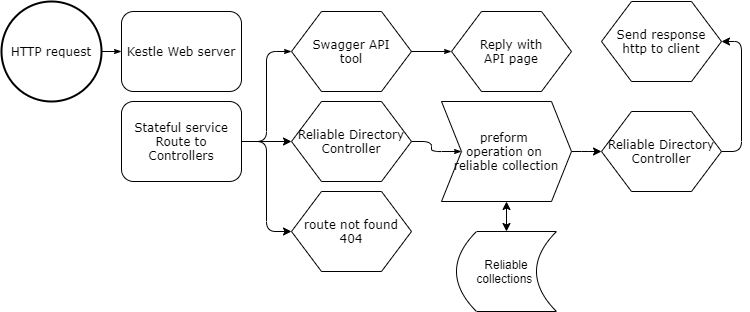
\includegraphics[scale=0.5]{images/Design_Stateful_service_1.0.drawio.png}

    This implementation contains 2 main codebases. The c\# dotnet web service that acts as a REST API to the reliable collections using 3 controllers for the 2 default data structures implemented in the framework, and a Clojure codebase that contains the test suite as well as an API connector, parsing, connections manager and fault handling..

    \subsubsection{Infrastructure}
    The infrastructure is centered around Azure, using a isolated v-net containing 6 virtual machines all running Linux, in this case Ubuntu was chosen as it's a known distribution that we are familiar with.1 of the 6 nodes is running the Jepsen application while the 5 other notes are running a Service Fabric Cluster.
    The 5 service fabric nodes are mostly self managing. Applications can be deployed via either the Azure Service Fabric CLI\cite{servicefabriccli} or via Visual Studio\cite{servicefabricguide} which was the process used doing the development stages of the project.

    This Jepsenhost is accessed via ssh and scp is used to deploy the newest version of the test code. Here a deployment pipeline could have been used to handle all of this by fetching, building and deploying via Jenkins or such a service but due to the goal of the project not being automated testing of Service Fabric, a bash script instead used that deployed code, started applications, ran the test and retrieve results.

    The topology of the network is simply just arrange such that the 6 nodes are located in the same VLAN to keep connections local and prevent outside connection to cause issues with the test.
    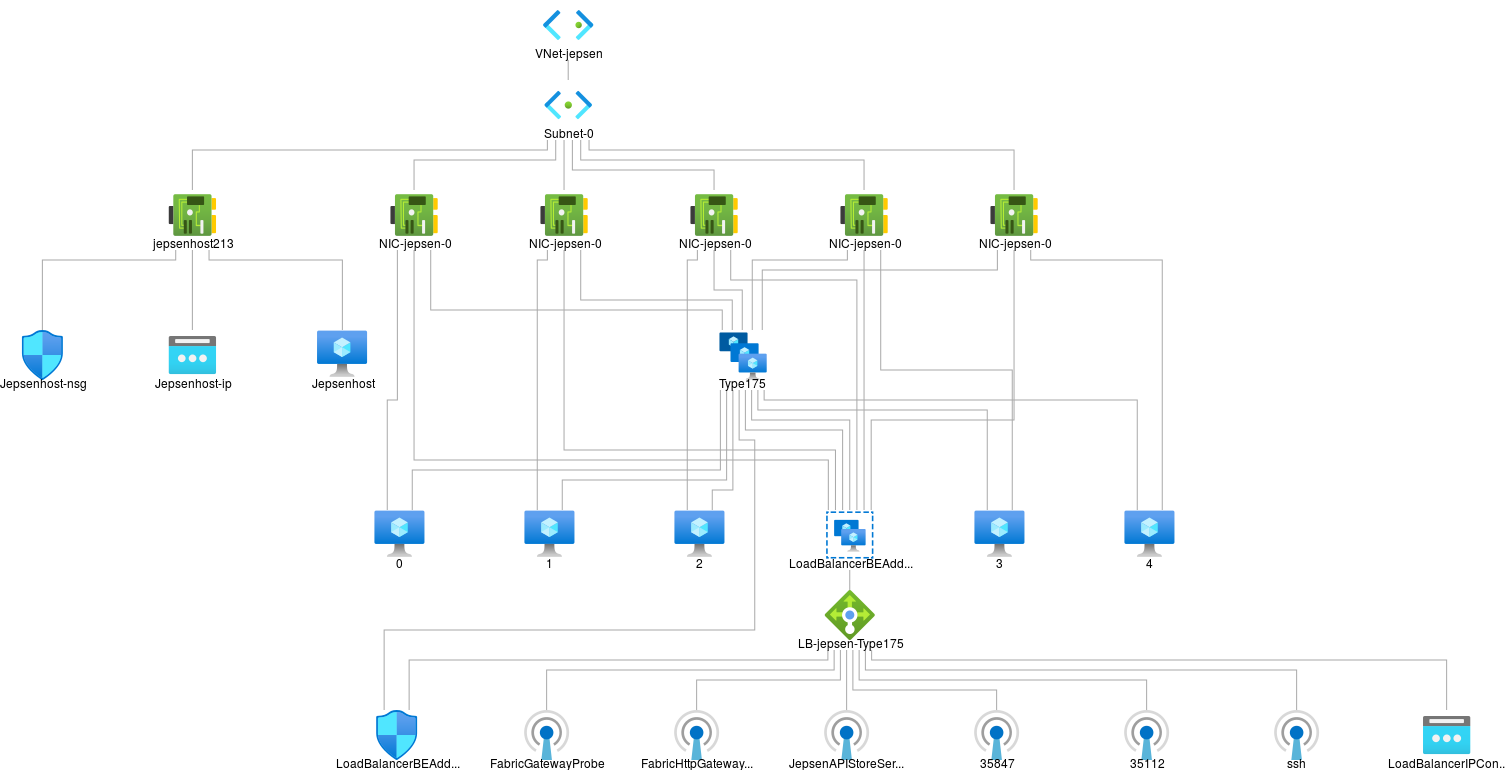
\includegraphics[scale=0.3]{images/topology.png}

    All traffic resides within the cluster and the load balancer is only there for testing of the application and check if all endpoints work as expected, These endpoint were protected by firewall rules that only allowed connections for the development address to avoid external influence of the results.

    \paragraph*{Node Sizes}

    The initial node sizes were 2 CPU cores and 8 GBs of ram along with 20 GB local storage, as this was thought be enough to handle the workload of the test. This was later revised as the nodes had issues with disk space and often took a long time to setup and get ready for any given deployment, this was resolved by upgrading the size of the nodes to 4vcpu, 16GB ram and 80GB local storage per node. This configuration resulted in a much more well-behaved cluster, and this node size was kept for the reminder of the test. However the Jepsenhost is slightly under-dimensioned compared to the workload it handles when computing on the result of the test. This is primary due to OOM errors that could be resolve with wither lowering the search space of the test or increasing the memory of the node itself.


    \section{Services}
    As mentioned earlier, running these tests required multiple components. The stateful service that hosts the reliable collections from SF Reliability subsystem, a restless front-end that provides this data to clients via REST API, a driver that handles the connection to this API and finally the Jepsen test suite itself consisting of both test suite and checker of the transactions and fault induced of the end system.

    \subsection{SF services}
    Using the 2 services approach as recommended from Microsoft provides multiple benefits but also a few negatives. the prime benefit it abstracting from the back-end and adding a layer of validation, routing, and protection of the back-end service. as well as greatly reducing the time that connections are held open to due RR times as all connections to the data store is kept within the cluster.

    \subsubsection{Stateful Reliable collection service}

    The stateful services provides 3 separate controllers that each provides one of the built in reliable collection types provided by service fabric. Reliable dictionary, reliable queue, and reliable concurrent queue. Fault handling is also handled at this stage where any fault stemming from the transactional issues is returned to the client via http status codes\cite{wikihttpstatuscodes}. eg node not primary, accepted, result not found.. etc.

    The fronted service simply provides these same APIs but with wrappers and routing in case of a portioned design. This layer could also be used to built additional features but this was not the case as only the bare transactions supported by the reliable collections layer was needed.

    \subsection{Jepsen test suite}
    The Jepsen test suite contains many layers and two main components a connector that connects to the service fabric services, and the test suite itself.

    The drive is the simplest service that is based on a raft API that was completely rewritten to interact with the SF API along with a custom fault handler that is able to parse both the result that the reliable collections API provides along with with the http codes in case something doesn't behave as intended.

    The Jepsen test component contains 6 classes. a runner, a db class that prepares for the test, a client that interacts with the driver, nemesis that induces faults in the cluster and 3 workloads, queue, cqueue, and dict. testing the 3 separate types provided by service fabric.

    The runner type is the main class that handles defaults, CLI input and test selection along with code that handles common behavior between the test. nemesis, db, along with other features that are mutual for all services that run in service fabric.

    the db class that is in charge for spinning up and tearing down the services along with functions for stating and stopping workers in the cluster.

    the nemesis class that contains the functions that kill, partition or otherwise mess and attempt to break the cluster.

    the 3 workloads.

    These each contain client for the test defining what endpoint to reach out to, a generator generating a sequence of transactions to preform on te database, and a checker that checks if our data stored behaved as expected.

    All types are expected to follow the repeatable-read consistently model. where the concurrent queue does best effort to meet the FIFO order of queued items compared the the normal queue following a FIFO ordering.

    \subsection{Implementation of the initial design}

    The initial designed first targeted the reliable collection dict datatype. and presented a few issues with the design and implementation details that was not considered.

    The biggest hurdle here was developing code for the service fabric Linux cluster due to a non feature parity between it and the windows cluster which caused non favorable conditions such as no debugging, binary dump files that weren't readable by any tool available.

    Here a great amount of time was spent debugging, changing configuration files, stripping any unneeded libraries and rolling back to older versions of frameworks. it should be noted that the service fabric framework was kept at the newest release while .NET and similar aspects where rolled back to older releases.

    All of these attempts were however frugal, after spending newly 2 months deleting all code, starting from scratch using a different skeleton code. trying the implementations via Java, going back to C\# getting a working solution on the windows service fabric implementation i reached out to Mikkel Hegnhøj from Microsoft.

    The issue turned out to be 2 fold.
    \begin{itemize}
        \item .NET needing to be rolled back to 3.5
        \item the entry point having to be defined via .NET and the name of the DLL file. this was something i attempt prior by using a entry point.sh that did the same while his solution was just replacing where the windows version has .exe with .DLL and as a .NET entry point.
    \end{itemize}

    Finally I had a runnable version on Linux, or rather. I had a way to run my application on Linux as the issues didn't stop here. The Feature parity was still there. The DNS was still missing, this required a lot of endpoints to be hard coded, which induced as one active replica of a given service per node. Eg. we can only have 1 service running per node which would greatly reduce horizontal scaling of the partitions which would greatly increase the number of partitions required to handling greater workloads. running larger partitions on each node is also an option but from a performance, availability, and reliability it's much effect having lots of smaller nodes instead of one large database instance that require a lot of broadcasting to each partition replica.


    This required some changes to the design but was resolved by removing of the layers in the application and accessing the stateful service directly, or rather creating a parallel service in case the other services were required later.

    \subsubsection{Implementation details SF}
        % The exact implementation of the service fabric services are covered in this section.
        %TODO this is broken. #cancer package
        % \lstinputlisting[language=csh, firstline=104, lastline=132, gobble=16, showstringspaces=false]{Jepsen/JepsenAPI/Controllers/ReliableDictionaryController.cs}
        
        
        The design uses a 2 service setup, the initial stateless service that processes the initial request and routes it to the back-end service. the read key call will be explained here but all the stateless endpoints work nearly identical to each other. so only one is included in the report.\\
        
        \paragraph{Stateless Service}
        The first first lines of code simply specify the URI of the function as well as what parts of the URI are parameters.
\begin{lstlisting}[language=csh]
// GET: uri:https://..../../api/.../key
[HttpGet("{key}")]
public async Task<IActionResult> Get(string key)
{
\end{lstlisting}   
Service Fabric reliable collections are very much a datatype in the hands of the developer, This wasn't entirely understood when starting out this project, but the reliable collections only expose a transactional storage engine, This requires of to first query to get a list of partions.
\begin{lstlisting}[language=csh]
    ServicePartitionList partitions = await this.fabricClient.QueryManager.GetPartitionListAsync(serviceName);
\end{lstlisting}   
And then enumerate the individual partitions, where some operations might require us to enumerated the values within each partition. 
\begin{lstlisting}[language=csh]
    foreach (Partition partition in partitions)
    {  .. Do something ..  }
    return this.Json(result);
\end{lstlisting}  

\paragraph{Statefull Service}

The stateful service was implemented with simplicity in mind that where each endpoint did one operation and committed this change to the database after some further consideration this approach was fairly flawed as it treats the system in the same manner that Base handles operations, however this realization wasn't made until much later is the process.

\begin{lstlisting}[language=csh]
        [HttpGet("{key}")]
        public async Task<IActionResult> Get(string key){
        ...
         while (await enumerator.MoveNextAsync(ct)){
                  if (enumerator.Current.Key == key)
                  { return this.Json(;(enumerator.Current);
    }}}
\end{lstlisting}   

    \subsubsection{Implementation details Clojure}
        For the implementation of the first deign for the Jepsen test a lot of things were a mess, due to a lot of considerations not having been made prior to writing the code and not fully understanding many of the underlying systems and learning a new programming language. which resulted in a board array of unintended and weird behavior, resulted from asynchronous distributed systems being complex and concurrent applications handling 100s, or 1000s of threads require planning and considerations where knowledge from concurrency theory should be used. 
        
        
        The Clujure application itself is split into a few different functions and classes. These are a runner, generator, Nemesis, db, client, connector/driver and workloads.
        \begin{itemize}
            \item         The runner contains the the majority of the configurations and a CLI interface that exposes options and settings where generalized values for the tests are specified. This is also where a select Workload is chosen for running the test. in total 3 different workloads were implemented that each require a generator, checker, client, and Nemesis.
        
        \item  The generator class generate a list of transaction to execute, which can later be used to check the transaction history for any anomalies. this is closely linked with the checker.
        
        \item  The checker checks the transaction history for anomalies.
        
        \item  the client interface maps Jepsen operations to API calls for our Service fabric Service and parses the result, and handles any faults that might have occurred doing the transaction.
        \end{itemize}
        
        
        For the Clojure application a few supporting libraries has to be written to allow it to interact with the API exposed by the Service Fabric applications. This connector was written in Clojure as well, It preforms a few different tasks mainly the HTTP/HTTPS calls, but also connection management, fault handling of connection, http, and server errors, as well as preparing and parsing information flowing both ways.
        
        

    \subsection{resolving issues with the design.}
    
    The initial version of the service fabric has some issues with the stateless service where the connection buffer simply overflew due to handling multiple connections for each incoming connection.

    The choice for solving this issue was simply to redesign the back-end service from the ground up. This revised service should simply provide a direct API from the stateful service, as the transactions are going to behave the same on a single partition compared to  a cluster with 500 partitions. the service is configured such that all replicas are active. this resolves and simplifies two things.  Routing is no longer an issue as our proxy node is removed, we no longer need to consider routing data to the correct node from our Clojure connector, where it's possible to route all traffic to the primary or only route writes to the primary possibly allowing for higher throughput.

    For the implementation a solution where all traffic is routed to the primary is simply selected as IO issues haven't yet been an issue.

    \subsection{Implementation of this design}

    The implementation of this revised design was supposed to be fairly straight forward, however the non feature parity poking it ugly head out again. Issues started showing up that was mainly due to a change in the release and forced update of a new version service fabric which change the behavior of some warning codes to instead cause errors. this exposed my inexperience working with the dotnet framework and the service fabric API. These issues were eventually ironed out but a lot of times was lost due to the lack of debugging support either from a local cluster or diagnostic output from the cluster itself which turned the development cycle upside down as I had no way to execute the code without service fabric but the code wouldn't run on service fabric cluster due to error code that lacked definition or documentation. The issue here ended up being related to changes in allowed port ranges that weren't allowed to be used by services and therefor the application where killed. These warnings were however not displayed correctly in the Linux distribution so tweaking code and settings was the only apparent solution for these issues.

    \subsubsection{Implementation changes for the SF Application}
    The second iteration of the design remove the stateless layer of the application however this approach was still flawed and was used for a large part of the initial project. it had the limitation that it was threatening the system with the eyes of the Base consistency model, This did show issues with the real tine constraint required by strict serializability or linearizability. \\
    
    The code changes to the service fabric aggregated the request handling from the stateless service into the stateful service along with changes to configurations to routing, request handling, and parsing.
    
    

    \subsubsection{Implementation changes for the Clojure Application}
        This design iteration didn't have any major changes on the Clojure application as the changes were on the routing side of service fabric. this did result in some changes on the connector that require spoofing to the headers on a internal service fabric application to avoid the request being rejected by the statefull application. Routing was also such that requsets were sent to the primary node by default.
    

\subsection{Final iteration of the design.}
    In this iteration the way transactions and calls between the client and server was changed, this required significant rewriting of the entire code project. due to the flawed approach in the 2 previous iterations.
    
    This required a full redesign of the way the request where handled such that the system used transactions and not just operations. The first design change is a new stateful service which needs to handle transactions containing a arbitrary long ordered list of operations to execute. and trivial compared to designing a new Jepsen test due to the way that the current Jepsen test generates, performs, parses, and checks the transaction history. 
    
    A change was also made to the network topology where all nodes were added to a proximity group that should reduce any latency or keep it to a minimal and ensure that outside forces such as bottle necked routing or switching gear aren't affecting the test results.  \\
    
    
    \paragraph{The Stateless service}
    
    
    The first first major change was changing the statefull API to support transactions. this required rebuilding the back-end to support this functionality which was greatly eased by using Postman, dotnetfiddle and curiousconcept json tools. but still extremely time consuming due to the lack of debug tools and generally black box behavior of Service Fabric, where issues weren't reproducible outside the cluster, and the cluster only returning internal server codes. The issue here turned out to be wrong documentation, which ended requiring a few days of investigation prior to being able to solve the issue. but it also summarizes the entire development process.\\
    \vspace{5mm}
    
    
    The revised backend recieves http calls where the transaction is included as a uri parameter containing json with the transaction in the following format\\
    \begin{lstlisting}[language=json]
{  "transaction":[
    {      "operation":"Enqueue",
     "key":"Key123",
     "value":456456    },
    {      "operation":"Dequeue",
     "key":"Key123"    },
    {      "operation":"abort"      }  ]}
    \end{lstlisting}  
    
    The revised backend unifies that endpoints into a single endpoint that takes a transaction as payload and executes this. 
    \begin{lstlisting}[language=csh]
[HttpPut]
public async Task<IActionResult> Put()
{
    IReliableDictionary<string, int> votesDictionary = await this.stateManager.GetOrAddAsync<IReliableDictionary<string, 
    ....
       foreach (var item in operationlist.transaction)
            {if (item.operation.Value == "r")
                {conditionalValue = await votesDictionary.TryGetValueAsync(tx, item.key.Value);
                        result.Add(new KeyValuePair<string, string>(item.key.Value, value.ToString()));}
            ....
     await tx.CommitAsync();
     return this.Json(result);}
\end{lstlisting}  

     \subsubsection{Implementation changes to the Jepsen Clojure application.}

The changes to the Jepsen application requiting starting anew and writing more functionality for the Jepsen service. Firstly was redoing the connector to use the new data types, parsing for the transactions to and from json, as well as the use of more complex generators and checkers for multi operation transaction. Elle was used as the underlaying package for some of this functionality with regards to generation and checking. The services such as the Client, db, connector etc required a bit more work code wise but less complex code compared to generation and checking.


\subsection{Running the code.}

    The test is run in Azure on a 5 node cluster with extra node outside the service fabric cluster for Orchestration of the test itself. deployment of the code to the cluster is pretty trivial and can be done either via Visual studio or a PowerShell script, The Jepsen test code is simply uploaded to the Orchestration node. From here the jepsen test can connect to the 5 nodes via SSH to induce crashes, time screws, and other failures and issues.
    
    Doing the test the systems take care of themselves and depending on the length of the test you can either remain connected and follow the tail of the output or reconnect at a later time to retrieve the results.


    \subsection{Issues that weren't resolvable}
    
    Linux and windows versions of the development environment being far from interchangeable with applications and services that function on windows and the local machine that fail to run or crash on cluster, this issue was further concatenated by visual studio being unable to load crash dump files that would allow a debugger to trace why the applications from the cluster weren't functioning as intended on the cluster. other debugging options such as the  Visual studio remote debugger feature wasn't compatible with the Linux cluster either which meant that the development was flying blind fairly often while developing. There was also some minor issues with the Cluster becoming unhealthy/corrupt and nodes not being configured correctly after a re-image that required a entire new deployment of the cluster and any data that might have been in the cluster to be lost. this was not an issue for the testing as the data wasn't of importance and was simply tractable data that could be used in the generated DSG and check for illegal edges in it.
    
    \section{Results}

    \subsection{Introduction}

    The results from the experiment with Jepsen and service fabric show a few things, the consistency model of Service fabrics reliable collections is pretty good, however there are some issues with regards to linearizability, and there a rather big caveat, the abort rate when transaction operate on multiple items in the distributed variables.
    
    It should be noted that concurrency wise Service fabric didn't do bad, but there are other aspects of the reliable collections that might pose issues when used without reading the fine grain of the documentation and having a good understanding of transaction models and what they allow.
    
    \subsection{Rejected transactions}
    
    One of the symptoms that the reliable collections showed was ever increasing abort rates for transactions containing more than 1 operation, These aborts were caused by heavy deadlocking and timeouts bringing the entire system to a slowdown with test containing randomly distributed transactions with 1-10 sub operations aborting 89.5 \% of the time meaning only 10.5 \% of the transaction got committed. The reason for these aborts resolves around the way that the API to service fabric is designed, that causing it to be blocking. The reliable collection doesn't preform any query optimizations, or any kind of checks prior to acquiring a lock or attempting to acquire them. 


    up to 10 operations per txn -> 89.5 \% Abort rate.
    :stats {:valid? true,
         :count 13086,
         :ok-count 1365,
         :fail-count 11721,
         :info-count 0,
         :by-f {:txn {:valid? true,
                      :count 13086,
                      :ok-count 1365,
                      :fail-count 11721,
                      :info-count 0}}},
                      
    ...
    with a txn lenght of max 3 of 32.9 \% Abort rate.
     :stats {:valid? true,
         :count 29225,
         :ok-count 19616,
         :fail-count 9609,
         :info-count 0,
         :by-f {:txn {:valid? true,
                      :count 29225,
                      :ok-count 19616,
                      :fail-count 9609,
                      :info-count 0}}},
                      
    \subsection{Lost writes or delayed writes.}
    
    The were occasions where writes seems to have disappeared, 
    
    
    
    \subsection{Violation of Strict Serializability}
    
    Some test showed violations of the Linearizability of the transactions. As Service fabric doesn't promise anything in terms of Linearizability, however some violations showed up doing the testing.




    \subsection{Not making use of optimizations}
    
    Service fabric doesn't make use of the optimizations available within service fabric, 
    
    No making use of many of the optimizations allowed within the consistency model that leaves a lot on the table.  


    \section{Discussion}

    \subsection{Violations of promised consistency level}

    Initially violation but was maybe due to network queue or other network issues?

    %TODO write introduction

    \subsection{Deeper issue}
    The topic of understanding transactional models possibly stems for the teaching of database systems and a lack of understanding what the different consistency models define, what they allow and how they behave in practice,

    %TODO Write Discussion Deeper issue
    The topic of understanding transactional models possibly stems for the teaching of database systems and a lack of understanding what the different consistency models define, what they allow and how they behave in practice,

    ....

    Going from this and other Jepsen tests on database it appears it's the issue is a board mislabeling and mis-classification of database systems and what they can and can't do.
    ...
    PostgresSQL replication and serializable,
    ...

    Going from this and other Jepsen tests on database it appears it's the issue is a board mislabeling and misclassification of database systems and what they can and can't do.
    ...
    PostgresSQL replication and serializable,
    ...

    MongoDB dropping data
    ...

    Casandra last-write wins, issues, and a attempt at a solution via Atomic clocks
    ...

    Elastic search issues.
    ...

    Some of the implications this can have on real world use cases,

    ...

    How to resolve these issues that aeries from mislabeled and misunderstood consistency models.

    ...

    Enable better understanding of databases, transaction models, and use cases doing teaching of database courses where behavior is better explained, This should not in depth but just to the level of read uncommitted or last-write-wins databases are fine for logging but should be avoided for most systems as they have a lot of unintended behavior, or at least theses systems should be below other layers that ensure that the data is persistent before a commit is accepted.

    ... should maybe be defined as future work.

    Whats next, Defining a standard for testing and certifying database systems towards transactional model that allows the industry to standardize the labelling and allows user and developers to choose the current system for their use case and avoid the headaches of phantom behavior.

    This could be done via automated testing and verification of a given system in it's different transactional configurations.


    \chapter{Conclusion and Outlook}
    \section*{Conclusion}
    %TODO write Conclusion
    
     I will only write deeper about designing, implementing, testing, executing and analysing the results. However this does not mean that the learning and understanding phase of the project was any smaller, quite the contrary. Learning 2 new programming languages that I've never interacted with before isn't an easy task; adding in the complexity of write code for cloud framework that I had no prior experience working on didn't help either. Spicing it with up with outdated documentation, incompatibility between versions of the framework and lack of debugging tools and broken tools meant that a lot was done via eyes blind brute forcing solutions to a lot of issues due to lacking features on the Linux version of the cluster.\\
     
     
    Whats next, Defining a standard for testing and certifying database systems towards transactional model that allows the industry to standardize the labelling and allows user and developers to choose the current system for their use-case and avoid the headaches of phantom behavior.

    This could be done via automated testing and verification of a given system in it's different transactional configurations.

    \section*{Outlook}
%TODO write Outlook


    \section{Future Work}
%TODO write Future Work
    Future work could include implementing a deeper testing suite that checks for more types of invariant and issues that might occur in the system.





    \newpage


    \chapter{Appendix}

    \pagestyle{empty}
    \printbibliography


    \section{Proposal}
    \section{'Jepsen methods usage for ACID compliance in Hyperscale Cloud Frameworks'}

\section{Introduction}
The goal of this project is to assess how Jepsen\footnote[1]{https://aphyr.com/tags/jepsen } tests allow us to verify the properties of ACID\footnote[2]{Database Management Systems by Raghu Ramakrishnan \& Johannes Gehrke  ISBN13 9780071231510} in a cloud system.
The Jepsen test is a method used to evaluate the compliance of a system in relation to the ACID properties. This is done is by analysing the system via Blackbox\footnote[3]{https://youtu.be/tRc0O9VgzB0?t=293} tests , in the sense that the internals of the system work are not relevant. We look at the service from a client-side and not any underlying structures or frameworks.
The ACID properties are 
\begin{itemize}
\item	Atomicity \\
Guarantees that each transaction is treated as a single "unit", which either succeeds completely or fails completely 
\item	Consistency \\
Ensures that a transaction can only bring the database from one valid state to another
\item	Isolation \\
Ensures that concurrent execution of transactions leaves the database in the same state that would have been obtained if the transactions were executed sequentially 
\item	Durability \\
Guarantees that once a transaction has been committed, it will remain committed even in the case of a system failure 
\end{itemize}
\footnote[2]{Database Management Systems by Raghu Ramakrishnan \& Johannes Gehrke  ISBN13 9780071231510} \\
We plan to apply these methods on Service Fabric\footnote[4]{https://docs.microsoft.com/en-us/azure/service-fabric/service-fabric-overview  } , to verify if this system is compliant with the ACID properties. Service Fabric is a framework developed by Microsoft, designed to allow developers to build Hyper-Scale Cloud (HSC) deployments on the Azure\footnote[5]{https://microsoft.com/en-us/azure/ } platform.
The motivation behind this thesis is to study the ACID properties in an HSC environment and evaluate how the constraints of ACID hold up in practice, as well as verifying if these constraints are met, and more importantly if they are not. 
\section{Plan}
     
The project is segmented into three parts. The writing of the report will take place at all times throughout the process, and the final phase should be a finalization and corrections phase.  
\subsection{The study phase  }
\begin{itemize}
\item	The first part of the study will focus on analysing the previous\footnote[6]{https://jepsen.io/analyses } Jepsen tests performed on other systems. This will allow us to define a strategy in terms of: which tools, tactics and methods are worth investigating, and what type of faults should be taken note of. This information is useful for two aspects:
\begin{itemize}
\item	where our focus should be when testing,  
\item	which tools and packages we should be familiarize with. 
\end{itemize}
\item	 The second part of the study will centre around “Service Fabric” and getting to know how the framework is coupled together, what vectors we can access the system from, and how we can manipulate the framework to induce fault conditions.   
\end{itemize}
\subsection{The experimentation phase}
\begin{itemize}
\item	In the experimentation phase, we will design and perform tests on the system. If any faults occur, we will attempt to locate where, and why they occur. If the scope and the timeline of the project allow, we will assess whether we prevent the faults from occurring in the future.
\item	The Experimentation phase of the project will include the steps described below. 
\begin{itemize}
\item	Planning of the test, selection of the aspects of the system to be tested, consulting with developers and users of the system to determine if and where undesired behaviour may occur.
\item	Designing the tests and setting up the tools to facilitate those tests.
\item	Writing the tests, verifying they work as intended and setting up a data collection framework to collect the data in a manner that allows our analysis.
\item	Performing the tests on the system in different scenarios, normal conditions and different levels of faults and disaster recovery.
\item	Analysing the data for faults, errors and inconsistencies.
\item	Consulting with DEVs to determine where the faults occurred, and which failures or bugs led to these fault conditions.
\item	Concluding whether “Service Fabric” is ACID-compliant. 
\end{itemize}
\end{itemize}
\subsection{The report phase }
\begin{itemize}
\item The final phase of the project aims at finishing an initial draft, reviewing and correcting it, and finalizing the report for hand-in.
\item	Deliverables 
\begin{itemize}
\item	At the end of the project, there should be a report, the tests and the results from those tests. 
\item	The report written in English and following the standard academic writing conventions will include 
\begin{itemize}
\item	A study on Jepsen tests, describing what they are, as well as why and how they are done.
\item	An experiment in which we will analyse “Service Fabric”	
\item	A discussion on the conclusiveness of the test and the compliance of the framework with service fabric.
\end{itemize}
\item	The code \& data will include
\begin{itemize}
\item	Scripts and code for tests and for analysing the data.
\item	Relevant results and data from the tests. 
\end{itemize}
\end{itemize}
\end{itemize}

\section{Goal}
The goal of the project is to deep dive into Jepsen tests with a focus on “Service Fabric” as the subject. The optimal goal of the project is to verify if the database aspects of “Service Fabric” comply with the ACID properties, and to locate the fault cases in case they don’t.    
Risk assessment 
There are a few risks in the project. In the case no faults are found within the Service Fabric, this reduces the scope of the project. If no faults are found, time allowing, different framework can be analysed. On the contrary, if the number of faults in the framework is more extensive than expected, then the scope of the project may grow uncontrollably. In this case, choices will be made to select a subset of the data to focus on.


    % \section{Schedule}

% Please add the following required packages to your document preamble:
% \usepackage{multirow}
% \usepackage[table,xcdraw]{xcolor}
% If you use beamer only pass "xcolor=table" option, i.e. \documentclass[xcolor=table]{beamer}

    % \begin{tabular}{clll}
    %     \multicolumn{2}{l}{Mark Jervelund thesis plan} & & \\
    %     & Week 45 &                                                    &                                                                                      \\
    %     & Week 46 &                                                    & \multirow{-2}{*}{\text{Study Jensen test}}                                           \\
    %     & Week 47 &                                                    &                                                                                      \\
    %     \multirow{-4}{*}{November} & Week 48 &                                                    & \multirow{-2}{*}{\text{Finish study on Jepsen test}}                                 \\
    %     & Week 49 &                                                    &                                                                                      \\
    %     & Week 50 &                                                    & \multirow{-2}{*}{\text{Study Service Fabric} }                                       \\
    %     & Week 51 &                                                    &                                                                                      \\
    %     & Week 52 &                                                    & \multirow{-2}{*}{\text{Christmas break}}                                             \\
    %     \multirow{-5}{*}{December} & Week 53 &                                                    &                                                                                      \\
    %     & week 01 & \multirow{-10}{*}{\text{Structured study 8 weeks}} & \multirow{-2}{*}{\text{Finish Study Service Fabric} }                                \\
    %     & Week 02 &                                                    &                                                                                      \\
    %     & Week 03 &                                                    & \multirow{-2}{*}{\text{designing the experiment}}                                    \\
    %     \multirow{-4}{*}{January}  & Week 04 &                                                    &                                                                                      \\
    %     & Week 05 &                                                    & \multirow{-2}{*}{\text{designing the experiment} }                                   \\
    %     & Week 06 &                                                    &                                                                                      \\
    %     & Week 07 &                                                    & \multirow{-2}{*}{\text{Execute the experiment}  }                                      \\
    %     \multirow{-4}{*}{February} & Week 08 &                                                    &                                                                                      \\
    %     & Week 09 &                                                    & \multirow{-2}{*}{\text{Analyse the experiment}}                                      \\
    %     & Week 10 &                                                    &                                                                                      \\
    %     & Week 11 & \multirow{-10}{*}{\text{Experiment 10 weeks}}      & \multirow{-2}{*}{\text{discover what the findings from the experiment is}}           \\
    %     & Week 12 &                                                    &                                                                                      \\
    %     \multirow{-5}{*}{March}    & Week 13 &                                                    & \multirow{-2}{*}{\text{Running additional experiments if needed Full on write mode}} \\
    %     & Week 14 &                                                    &                                                                                      \\
    %     & Week 15 &                                                    & \multirow{-2}{*}{\text{Full on write mode} }                                         \\
    %     & Week 16 &                                                    &                                                                                      \\
    %     \multirow{-4}{*}{April}    & Week 17 &                                                    & \multirow{-2}{*}{\text{Full on write mode} }                                         \\
    %     & Week 18 &                                                    &                                                                                      \\
    %     & Week 19 &                                                    & \multirow{-2}{*}{\text{Full on write mode Send out thesis for feedback}}             \\
    %     & Week 20 &                                                    &                                                                                      \\
    %     & Week 21 & \multirow{-10}{*}{\text{Thesis writing 10 weeks}}  & \multirow{-2}{*}{\text{Correction} }                                                 \\
    %     \multirow{-5}{*}{May}      & Week 22 &                                                    &                                                                                      \\
    %     & Week 23 & \multirow{-2}{*}{\text{goal}}                      & \multirow{-2}{*}{\text{Hand in}}                                                     \\
    %     & Week 24 & \multicolumn{1}{l}{}                               & \multicolumn{1}{l}{}                                                                 \\
    %     & Week 25 & \multicolumn{1}{l}{}                               & \multicolumn{1}{l}{}                                                                 \\
    %     & Week 26 & \multicolumn{1}{l}{}                               & \multicolumn{1}{l}{}                                                                 \\
    %     \multirow{-5}{*}{June}     & Week 27 & \multicolumn{1}{l}{}                               & \multicolumn{1}{l}{}                                                                 \\
    %     \multicolumn{1}{l}{}       & Week 28 & \multicolumn{1}{l}{}                               & \multicolumn{1}{l}{}                                                                 \\
    %     \multicolumn{1}{l}{}       & Week 29 & \multicolumn{1}{l}{}                               & \multicolumn{1}{l}{}                                                                 \\
    %     \multicolumn{1}{l}{}       & Week 30 & \multicolumn{1}{l}{}                               & \multicolumn{1}{l}{}                                                                 \\
    %     \multicolumn{1}{l}{}       & Week 31 & \multicolumn{1}{l}{}                               & \multicolumn{1}{l}{}
    % \end{tabular}

\end{document}